\section{The $VH (H \rightarrow b\bar{b}/c\bar{c})$ Combined Analysis}
\subsection{Introduction}
Perhaps the most important  \textit{raison d'être} of the \textit{Large Hadron Collider} (LHC) was to discover the Brout-Englert-Higgs boson (Higgs - $H$), a feat achieved by the ATLAS and CMS Experiments in July 2012 \cite{ATLAS:2012yve, CMS:2012qbp}. Theorised in 1964 by two independent papers introducing the mechanism of spontaneous symmetry breaking to give mass to the gauge bosons \cite{Englert:1964et,  PhysRevLett.13.508}, its discovery almost forty years later marked one of the greatest achievements of the particle physics community. The Higgs boson is an essential part of the SM as it is tied to the mechanism through which particles acquire mass without breaking the electroweak gauge invariance. \\

Since then, both experiments have been studying the specific properties of the discovered particle, and in particular the different production processes and decay channels. During the LHC Run 2, corresponding to data taken from 2015 to 2018, the $t\bar{t}H$ production mechanism was observed for the first time \cite{ATLAS:2018mme, CMS:2018uxb}. The decay channel of the Higgs boson to a $b\bar{b}$ pair was observed \cite{ATLAS:2018kot, CMS:2018nsn} and there now is evidence of the decay to a $\mu^-\mu^+$ pair \cite{ATLAS:2020fzp, CMS:2020xwi}. The former decay channel is of significance since it has the largest predicted branching ratio of 58\% for $m_H = 125$ GeV. The latter is the first evidence of the decay of the Higgs to second-generation fermions. Furthermore, constraints on the branching ratio of the $H$ to another second-generation fermion, the $c$-quark, have been set by both collaborations studying the $H \rightarrow c\bar{c}$ decay \cite{Aaboud:2018fhh}. This decay mode is the most common Higgs decay mode that has yet to be observed. It is indeed particularly challenging due to the small predicted branching ratio of 2.89\% compared to $H \rightarrow b\bar{b}$, the large background rate, and the experimental difficulties in identifying $c$-jets. It is a fertile ground for new physics beyond the SM as well as an important test of the validity of the model. The fermion couplings in the SM were indeed added ad-hoc and there is a distinct mass hierarchy between the three generations of quarks that can be probed by studying their coupling strengths to the Higgs boson. In the $VH (H \rightarrow b\bar{b}/c\bar{c})$ analysis, the hierarchy of mass between the $b$- and $c$-quark, respectively a $3^{\textrm{rd}}$ and $2^{\textrm{nd}}$ generation quark, is probed.

\subsection{The $VH (H \rightarrow b\bar{b}/c\bar{c})$ analyses in ATLAS}
While $H \rightarrow b\bar{b}$ enjoys the largest branching ratio at the observed Higgs mass, the large multi-jet background in a hadron collider like the LHC makes this decay mode very challenging. The measurements for both the $b\bar{b}$ and $c\bar{c}$ decay modes are therefore performed in a so-called \textit{associated production mode}, where the $H$ is produced in addition with an extra vector boson $V$ ($W$ or $Z$) decaying leptonically, to electrons ($e$), muons ($\mu$), neutrinos ($\nu$), or a combination $e\nu$ or $\mu\nu$. Taus ($\tau$) are not included at the moment though some tests are being run to add them, in particular, to migrate 0L-channel events with a hadronically decaying $\tau$ to the 1L channel. Despite the relatively small cross-section of the $VH$ production mode ($\sigma_{VH}$ = 2.25 pb compared to the total $H$ production $\sigma_H \approx$ 51 pb), the process benefits from experimentally favourable conditions thanks to the presence of leptons in the event signature: these allow for efficient triggering, the act of rapidly deciding whether to further process and store an event when collecting the data, and greatly reduce the contribution of the multi-jet background. \\

In the ATLAS collaboration, the $VH (H\rightarrow b\bar{b})$ and $VH (H\rightarrow c\bar{c})$ analyses adopt very similar strategies, with the main ingredient being the ability to reliably tag the flavour of jets produced in an event, thereby reconstructing the heavy quark pair produced in the $H$ decay. Using the full Run 2 dataset, the published ATLAS analysis obtained the following upper limits on the signal strength of the $VH (H\rightarrow c\bar{c})$ as predicted by the SM: an observed (expected) upper limit of 26 $\times$ SM (31 $\times$ SM) \cite{Collaboration:2721696}. For comparison, CMS reported an observed (expected) upper limit of 14 $\times$ SM (7.6 $\times$ SM) \cite{arXiv:2205.05550}. \\ 

For the $VH (H\rightarrow b\bar{b})$, thanks to a larger expected signal, the analysis reaches a sensitivity of 6.7 standard deviations \cite{ATLAS:2020fcp}. Therefore, more detailed measurements can be made, such as the cross-section as a function of momentum in the reduced Simplified Template Cross-Section (STXS) scheme. To probe larger $p_T$ ranges, the analysis is now split into the \textit{resolved} \cite{ATLAS:2020fcp} and \textit{boosted} \cite{ATLAS:2020jwz} analyses, with the latter restricting to values of the transverse momentum of the associated vector boson $p_T^V$ above 250 GeV. The name of these analyses comes from the ability to independently resolve the two $b$-jets into two distinct small cone radius (small-$R$) jets at low $p_T^V$. At high $p_T^V$, the Higgs $p_T^H$ is highly Lorentz-boosted and a single large-radius ($R = 1$) jet, merging the two $b$-jets, can be reconstructed as a candidate for the Higgs. The measured signal strengths, the ratio of the measured yield to the SM predictions, are: 
\begin{itemize}
\item For the resolved analysis in Run 2: a signal strength of $1.02_{-0.17}^{+0.18}$ corresponding to an observed (expected) significance of 6.7 (6.7) standard deviations \cite{ATLAS:2020fcp}. Due to the good sensitivity of the analysis, the result is further detailed into the $WH$ and $ZH$ production processes with observed (expected) significances of, respectively, 4.0 (4.1) and 5.3 (5.1) standard deviations. Furthermore, the $VH$ cross-section times the $H \rightarrow b\bar{b}$ and $V\rightarrow$ leptons branchings fractions ($\sigma \times BR$) are reported in the reduced STXS scheme. Finally, limits are set on the coefficients of effective Lagrangian operators which can affect the $VH$ production and the $H \rightarrow b\bar{b}$ decay.
\item For the boosted analysis: a signal strength of  $0.72_{-0.36}^{+0.39}$ corresponding to an observed (expected) significance of 2.1 (2.7) standard deviations \cite{ATLAS:2020jwz}.
\end{itemize}

It is interesting to note that the combination has already been tested for the resolved $VH (H\rightarrow b\bar{b})$ + $VH (H\rightarrow c\bar{c})$ \cite{Collaboration:2721696} and the resolved + boosted $VH (H \rightarrow b\bar{b})$ \cite{ATLAS:2021wqh}. However, these used the published analyses and the objective of the new Combined Analysis is to define a common analysis strategy for both Higgs decay modes, thereby improving the measurements of $VH (H \rightarrow b\bar{b})$ and $VH (H \rightarrow c\bar{c})$ simultaneously. This combined measurement has several additional benefits: 
\begin{itemize}
\item The Higgs-charm and -beauty coupling modifiers $\kappa_c$ and $\kappa_b$ can be measured directly, as well as their ratio $\kappa_c/\kappa_b$. 
\item The auxiliary measurements of background processes are shared, leading to a better knowledge of background processes that contribute to both phase spaces such as the $V$+jets and top-quark processes.
\end{itemize}

The rest of this section focuses on the current state of the $VH (H\rightarrow c\bar{c})$ part of the Combined Analysis, as the analysis is not yet concluded. 

\subsection{Analysis strategy}
The Combined Analysis is performed with the full ATLAS Run 2 proton-proton collision data, from 2015 to 2018, for a total integrated luminosity of 140 fb$^{-1}$ at a centre of mass energy $\sqrt{s} = 13$ TeV. The regions and boundaries between the different regimes of the analysis are illustrated in Figure \ref{fig:ana-strat}. The separation is based on jet flavour tagging (for  $VH (H\rightarrow b\bar{b})$ and $VH (H\rightarrow c\bar{c})$) and on a $p_T^V$ cut of 400 GeV (for the resolved - boosted  $VH (H\rightarrow b\bar{b})$). The $(\rightarrow b\bar{b})$ - $(\rightarrow c\bar{c})$ analyses are separated by the required presence of two $b$-tagged jets or a $c$-tagged jets respectively. The $p_T^V$ cut marks the difference between the Higgs candidate reconstruction scheme: two small radius (R = 0.4) jets below a $p_T^V$ of 400 GeV and one large radius (R = 1) jets with two sub-jets above.

\begin{figure}[h!]
\center
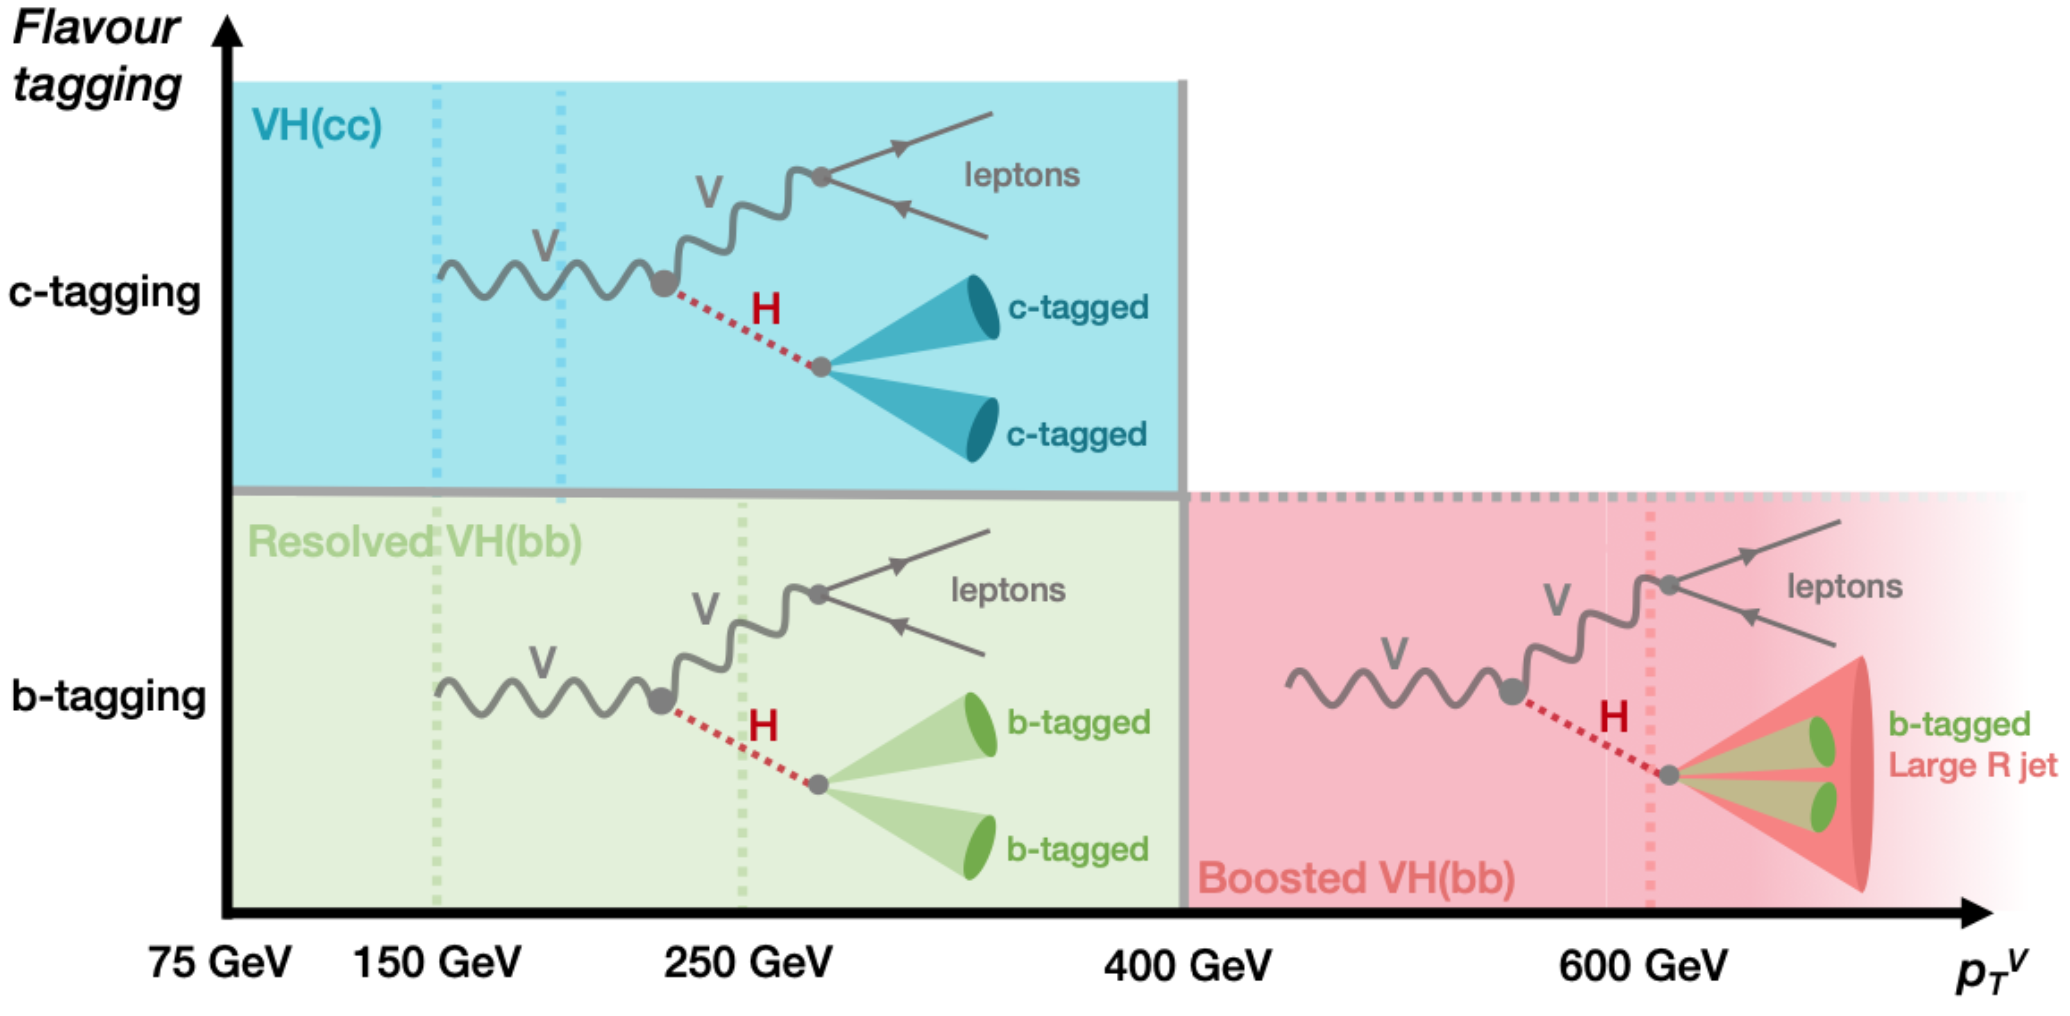
\includegraphics[scale=0.35]{Images/VH/AnalysisRegime.png}
\caption{The analysis regimes considered in the $VH (H\rightarrow b\bar{b}/c\bar{c})$ analysis, from the internal documentation of the team \cite{Chisholm:2743096}.} 
\label{fig:ana-strat}
\end{figure}

For all analysis regions, three different channels are defined based on the decay mode of the vector boson $V$: $Z \rightarrow \nu \nu$ (\textit{0-lepton} - 0L), $W \rightarrow l \nu $ (\textit{1-lepton} - 1L), and $Z \rightarrow l^+ l^-$ (\textit{2-lepton} - 2L), where $l$ refers to an electron or a muon and $\nu$ to any type of neutrino. The signal considered are the  $VH (H\rightarrow b\bar{b})$ and $VH (H\rightarrow c\bar{c})$ processes. The SM diboson processes $VZ (Z\rightarrow b\bar{b})$ and $VZ (Z\rightarrow c\bar{c})$ are considered as signals in a cross-check analysis. Having a larger cross-section, these processes kinematically similar to the signals can be measured with good statistical significance, thereby offering a suitable test case to verify the performance of the strategy deployed. The main backgrounds are the $V$+jets (mostly $Z$+jets in 0L and 2L, $W$+jets in 1L) and top-quark processes (predominantly the top-quark pair production $t\bar{t}$, with one of the $t$ decaying leptonically, and a sub-leading contribution from single top-quark production, both in 0L and 1L). Minor backgrounds are the multi-jet (thanks to the required presence of leptons) and diboson pair productions ($VV$). All backgrounds are simulated using Monte Carlo (MC) simulation packages, except for the multi-jet which is estimated from a data-driven method in the 1L channel and is negligible in other channels. To reproduce the conditions of the ATLAS detector, simulated samples are passed through the GEANT4 software \cite{Agostinelli:602040} and the ATLAS reconstruction software.

\subsubsection{Objects description}
When a particle passes through the ATLAS detector, different types of electronic signals are collected by the various sub-detectors. This raw information is then processed in successive computational steps to reconstruct high-level physics objects that are then used by analyses. For the particular $VH (H\rightarrow c\bar{c})$ analysis, the most important objects are:
\begin{itemize}
\item Jets: calorimeter jets with a radius $R$ = 0.4 reconstructed with the Particle Flow and anti-$k_t$ algorithms \cite{Cacciari:2008gp} are used. A jet is considered as \textit{signal} if it has a $p_T$ > 20 GeV and $|\eta| < 2.5$. It is considered as \textit{forward} if 2.5 $\leq |\eta|$ < 4.5, with a $p_T > 30$ GeV. Because the Higgs candidates are selected based on the tagged flavour and the tagger works up to $|\eta| = 2.5$, due to its reliance on the tracking detectors, only signal jets are considered as candidates. To suppress pile-up jets, which is predominately made of light-jets, a 30 GeV $p_T$ is applied to all non-Higgs candidate jets. For the Higgs candidates, the lower $p_T$ threshold of 20 GeV is kept, as flavour tagging suppresses most of these light-jets. 
\item Electrons: identified with a likelihood-based method matching a deposit in the electromagnetic calorimeter with a track \cite{Aaboud:2657964}. Requirements are summarised in Table \ref{tbl:elOb} and vary depending on the lepton channel. A $VH$-Loose with loose likelihood identification is applied to electrons in all channels. Additionally, the $ZH$-Signal and $WH$-Signal criteria are applied in the 1L and 2L channels respectively, with a tighter $p_T$ due to the trigger threshold. The 1L likelihood identification and isolation selections are tighter to suppress the multi-jet background.
\item Muons: reconstructed by matching an energy deposit in the muon detector with information from the Inner Detector and Muon Spectrometer \cite{Aad:2746302}. Requirements are summarised in Table \ref{tbl:muonOb} and vary depending on the lepton channel. The $VH$-Loose requirement is applied to muons in all channels. The $ZH$-Signal and $WH$-Signal are additionally applied to the 1L and 2L channels respectively. 
\item $E_T^{\textrm{miss}}$ (MET): neutrinos are not detectable in ATLAS and their presence can be inferred from momentum imbalance in the transverse plane. $E_T^{\textrm{miss}}$ is the negative vectorial sum of the $p_T$ of physics objects (leptons, jets, ...) as well as a track-based \textit{soft term}, introduced to include a contribution from good quality tracks not associated to a main physics object.
\item Taus: hadronically decaying tau-leptons are identified and vetoed in 1L using a recurrent neural network (RNN) \cite{ATL-PHYS-PUB-2019-033}. In 0L and 2L, if the jet passes the RNN requirement for hadronically decaying tau-leptons, it is no longer considered as a jet and cannot be considered as a Higgs candidate. 
\end{itemize}

\begin{table}[!htbp]
  \begin{center}
    \resizebox{0.95\textwidth}{!}{
      \begin{tabular}{ccccccc} \hline \hline
        Electron Selection & $p_T$ & $\eta$ & ID & $d_{0}^{\mathrm sig}$ w.r.t. BL &  $|\Delta{z_{0}}\sin\theta|$ & Isolation \\ \hline
        VH-Loose & $>$7 GeV & $|\eta|< 2.47$ & LH Loose & $ <5$ & $<0.5$ mm & Loose\_VarRad \\
        ZH-Signal & $>$27 GeV & \multicolumn{5}{c}{Same as VH-Loose} \\
        WH-Signal & \multicolumn{2}{c}{Same as ZH-Signal} & LH Tight & \multicolumn{2}{c}{Same as ZH-Signal} & HighPtCaloOnly \\
        \hline\hline
      \end{tabular}
    }
    \caption{Electron Selection}
    \label{tbl:elOb}
  \end{center}
\end{table}

\begin{table}[!htbp]
\vspace{-1cm}
  \begin{center}
    \resizebox{0.95\textwidth}{!}{
      \begin{tabular}{ccccccc} \hline \hline
        Muon Selection & $p_T$ & $\eta$ & ID & $d_{0}^{\mathrm sig}$ w.r.t. BL  & $|\Delta{z_{0}}\sin\theta|$ & Isolation \\ \hline
        VH-Loose & $>$7 GeV & $|\eta|< 2.7$ & Loose quality & $ <3$ & $<0.5$ mm & Loose\_VarRad \\
        ZH-Signal & $>$27 GeV & $|\eta| < 2.5$ & \multicolumn{4}{c}{Same as VH-Loose} \\
        %WH-Signal & $>$25 GeV ($>$27 when $p_T^V<$ 150 GeV) & $|\eta|< 2.5$ & Medium quality & $ <3$ & $<0.5$ mm & HighPtTrackOnly \\
        WH-Signal & \makecell[c]{$>$25 GeV when $p_T^V>$ 150 GeV\\ $>$27 GeV when $p_T^V<$ 150 GeV} & $|\eta|< 2.5$ & Medium quality & $ <3$ & $<0.5$ mm & HighPtTrackOnly \\
        \hline\hline
      \end{tabular}
    }
    \caption{Muon Selection}
    \label{tbl:muonOb}
  \end{center}
\end{table}

\vspace{-1cm}

\subsubsection{Event categorisation}
Events are categorised following a decomposition into regions of specific flavour-tags, $p_T^V$ range, number of jets, and cuts on the $\Delta R$ between the Higgs candidate jets. As  $VH (H\rightarrow b\bar{b})$ is completely orthogonal to $VH (H\rightarrow c\bar{c})$, the event categorisation of the boosted analysis is not described here.

\paragraph{Flavour tagging:} Jet flavour tagging is perhaps the most important part of the analysis. The DL1r algorithm is used and calibrated for the analysis for both $b$- and $c$-tagging. At the time of the analysis, the superior DL1d and GN1 taggers of the previous section were not yet available and their calibration is an ongoing effort. The $VH$ analyses require extensive flavour-tagging and an in-depth study of the numerous and important backgrounds and their flavour components. This takes a significant amount of work, making a switch to a new tagger not feasible from a practical point of view in the timing of the analysis. They represent, however, an exciting avenue for progress in future iterations of this search. The \textit{Pseudo-Continuous Flavour Tagging} scheme (PCFT), shown in Figure \ref{fig:pseudotag}, is employed for a coherent joint definition of $b$- and $c$-tagged jets. For a given jet, it is first decided whether the jet is $b$-tagged ($B$), based on a $b$-tagging working point with 70\% efficiency. These working points are derived on a set of calibrating samples: dileptonic $t\bar{t}$ for $b$-jets, semileptonic $t\bar{t}$ for $c$-jets, and $Z$+jet samples for light-jets. If the $b$-tagging requirement is not met, it is then considered whether the jet is $c$-tagged using the same DL1r tagger at a working point defined and calibrated in the context of the analysis. A \textit{loose} ($L$) and \textit{tight} ($T$) $c$-tagging requirements are defined, each at an exclusive $c$-tagging efficiency of 20\%. Being made of the top tier $c$-jets, the $b$- and light-rejections of the tight $c$-tagging working point are improved compared to the looser working point. The $c$-jet (light-jet) efficiency in the $b$-tagged bins of the PCFT scheme is 7.85\% (0.181\%) and the $b$-jet (light-jet) efficiency in the loose $c$-tagged ($L$) bin is 11.5\% (6.5\%) while it is 4.5\% (0.9\%) in the tight $c$-tagged bin ($T$). Jets that are not tagged are ascribed the letter $N$. \\

\begin{figure}[h!]
%\hspace{-2.0cm}
\center
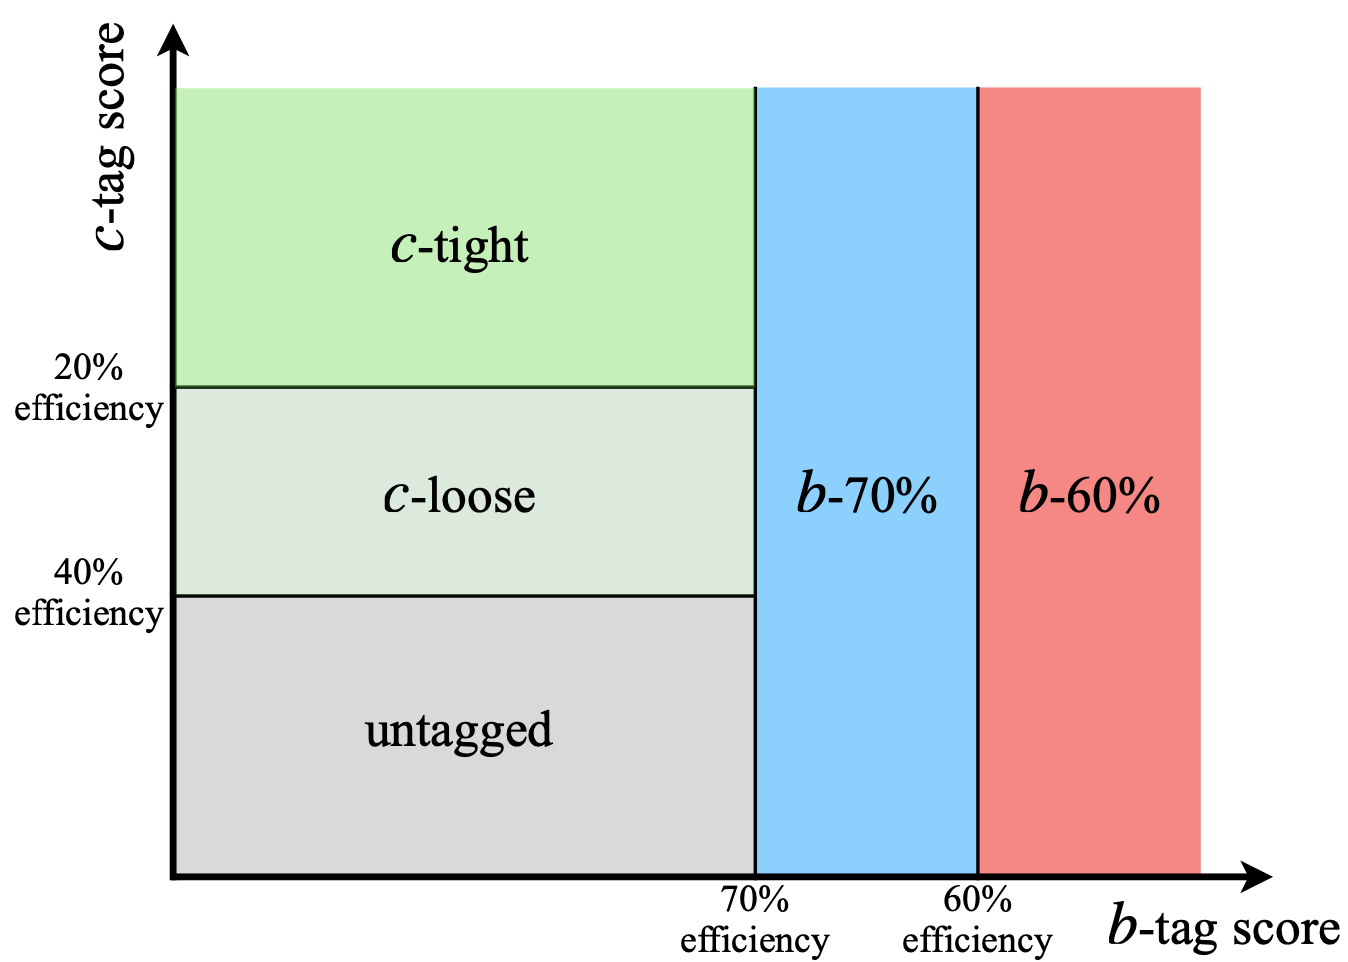
\includegraphics[scale=0.45]{Images/VH/pseudocontinuous.png}
\caption{The pseudo-continuous tagging scheme, from the internal documentation of the team \cite{Chisholm:2743096}. } 
\label{fig:pseudotag}
\end{figure}

In an event with at least two signal jets, the candidate jets selected to reconstruct the Higgs define an event-tag by combining their individual tags. While in the past the so-called \textit{Leading 2-jet} strategy was used, where the candidate jets were the two highest $p_T$ signal jets, a new strategy called \textit{All Signal Jets} is now preferred in the $VH$ analysis as it improves the expected statistical significance. The strategy introduces a hierarchy of tags: $B$ > $T$ > $L$ > $N$. The pair of candidates is made of the two signal jets having the highest tags, and, in case of ties, the highest $p_T$. The tagging requirements for an event to be in the signal regions (SR) are:
\begin{itemize}
\item For $VH(H\rightarrow b\bar{b})$, strictly two jets must be $b$-tagged and no tight $c$-tagged jets are allowed. 
\item For $VH(H\rightarrow c\bar{c})$, no $b$-tagged jets are allowed and at least one jet must be tight $c$-tagged. This defines three possible signal regions, where a second jet is either tight $c$-tagged ($TT$), loose $c$-tagged ($LT$), or not tagged ($TN$). 
\end{itemize}

Two control regions are defined by modifying the conditions on the tags of the jets in the event: 
\begin{itemize}
\item A combined $VH(H\rightarrow b\bar{b})$ and $VH(H\rightarrow c\bar{c})$ top control region (topCR) is obtained by requiring at least 1 $b$-tagged jet and 1 $c$-tagged jet. The definition of this control region is the core subject of this work and will be further addressed later in this report. 
\item For $VH(H\rightarrow c\bar{c})$ only, an additional control region is defined by requiring no $b$- nor $c$-tagged jets in the event to constrain the significant $V$+light-jet background. 
\end{itemize}

\paragraph{Ranges of $p_T^V$:} The categorisation is made of the following $p_T^V$ regions in the non-boosted regime:  $[150, 250]$ GeV and $[250, 400]$ GeV. For the 2L channel only, a low $p_T^V \in [75, 150]$ GeV is included - this is not feasible in 0L due to the trigger threshold on MET nor in 1L as the large amount of background at low $p_T$ means this region does not improve the statistical significance.

\paragraph{Number of jets:} Every region is split between a 2-jet and a 3-jet region, except for the 2L channel where events with 3 or more jets are included in the 3-jet region as there is almost no $t\bar{t}$ background thanks to the two leptons and $c$-jets requirements. In 0L and 1L, there is a large amount of $t\bar{t}$ background in the 4J region, hence the tighter requirement. Including this potential higher jets number region was observed to not improve the statistical significance. 

\paragraph{$\Delta R$ between the jets:} the angular separation between the two candidate jets $\Delta R(j_1, j_2)$, as defined in Equation \ref{eq-deltaR}, can be used to define a control region enriched in $V$+jets and $t\bar{t}$ backgrounds since these two processes give candidate jets with a flat angular spectrum while the signal peaks at low values of $\Delta R$. 

\begin{equation}\label{eq-deltaR}
\Delta R(j_1, j_2) = \sqrt{(\eta_{j_1} - \eta_{j_2})^2 + (\phi_{j_1} - \phi_{j_2})^2 }
\end{equation}

A \textit{high $\Delta R$} control region (High $\Delta R$ CR) is defined using parametrised cuts on $\Delta R$ between the Higgs candidate jets as a function of $p_T^V$. An additional \textit{low $\Delta R$} control region (Low $\Delta R$ CR) for the 1L channel in $VH (H\rightarrow b\bar{b})$ resolved is also introduced (it is merged with the signal region for the $VH (H\rightarrow c\bar{c})$). The philosophy behind the parametrisation of this function is to adapt the cut on the expected angular separation between the two Higgs candidate jets as a function of how boosted they are, as described by the $p_T^V$ variable. For signal events, we expect the $H$ and $V$ to be approximately back-to-back hence $p_T^V$ is a good proxy for $p_T^H$ while benefiting from better experimental resolution, as it is reconstructed from leptons $p_T$ and/or $E_T$, depending on the channel. From physical principals, boosted candidate jets are indeed expected to have a lower angular separation. From the point of view of $VH (H\rightarrow c\bar{c})$, this modified cut represents a significant modification to the standalone analysis that relied on a simple fixed $\Delta R_{c\bar{c}}$ cut. The new cuts are defined by fitting a template function $ c_1 \times e^{c_2 + c_3 \times p_T^V}$ so that:   
\begin{itemize}
\item 95\% (85\%) of the $VH(H\rightarrow c\bar{c})$ signal is below the top limit for the 2-jet (3-jet) signal region,
\item 90\% of the diboson process is above the bottom limit in both signal regions.
\end{itemize}

The results of these fits for the 1L channel are displayed in Figure \ref{fig:drccptvCutsVHcc}, showing the signal yield in a 2-dimensional histogram ($p_T^V$ vs $\Delta R_{c\bar{c}}$) for different tags applied. The cut used in $VH(H\rightarrow b\bar{b})$, in yellow, shows a good agreement with the one derived on the $TT$-tagged (tight-tight) events in cyan and the $LT$-tagged (loose-tight) in green. The $VH(H\rightarrow b\bar{b})$ cuts is chosen so that the kinematic selection of the two analyses is harmonised. In $VH (H\rightarrow c\bar{c})$, the low $\Delta R$ CR does not improve the statistical significance hence this region is merged with the signal region. In $VH(H\rightarrow b\bar{b})$, these CRs are used to extract the normalisation of the backgrounds while in $VH (H\rightarrow c\bar{c})$ the shape of the $m_{c\bar{c}}$ spectrum is also used.  \\

\begin{figure}[h!]
%\hspace{-2.0cm}
\center
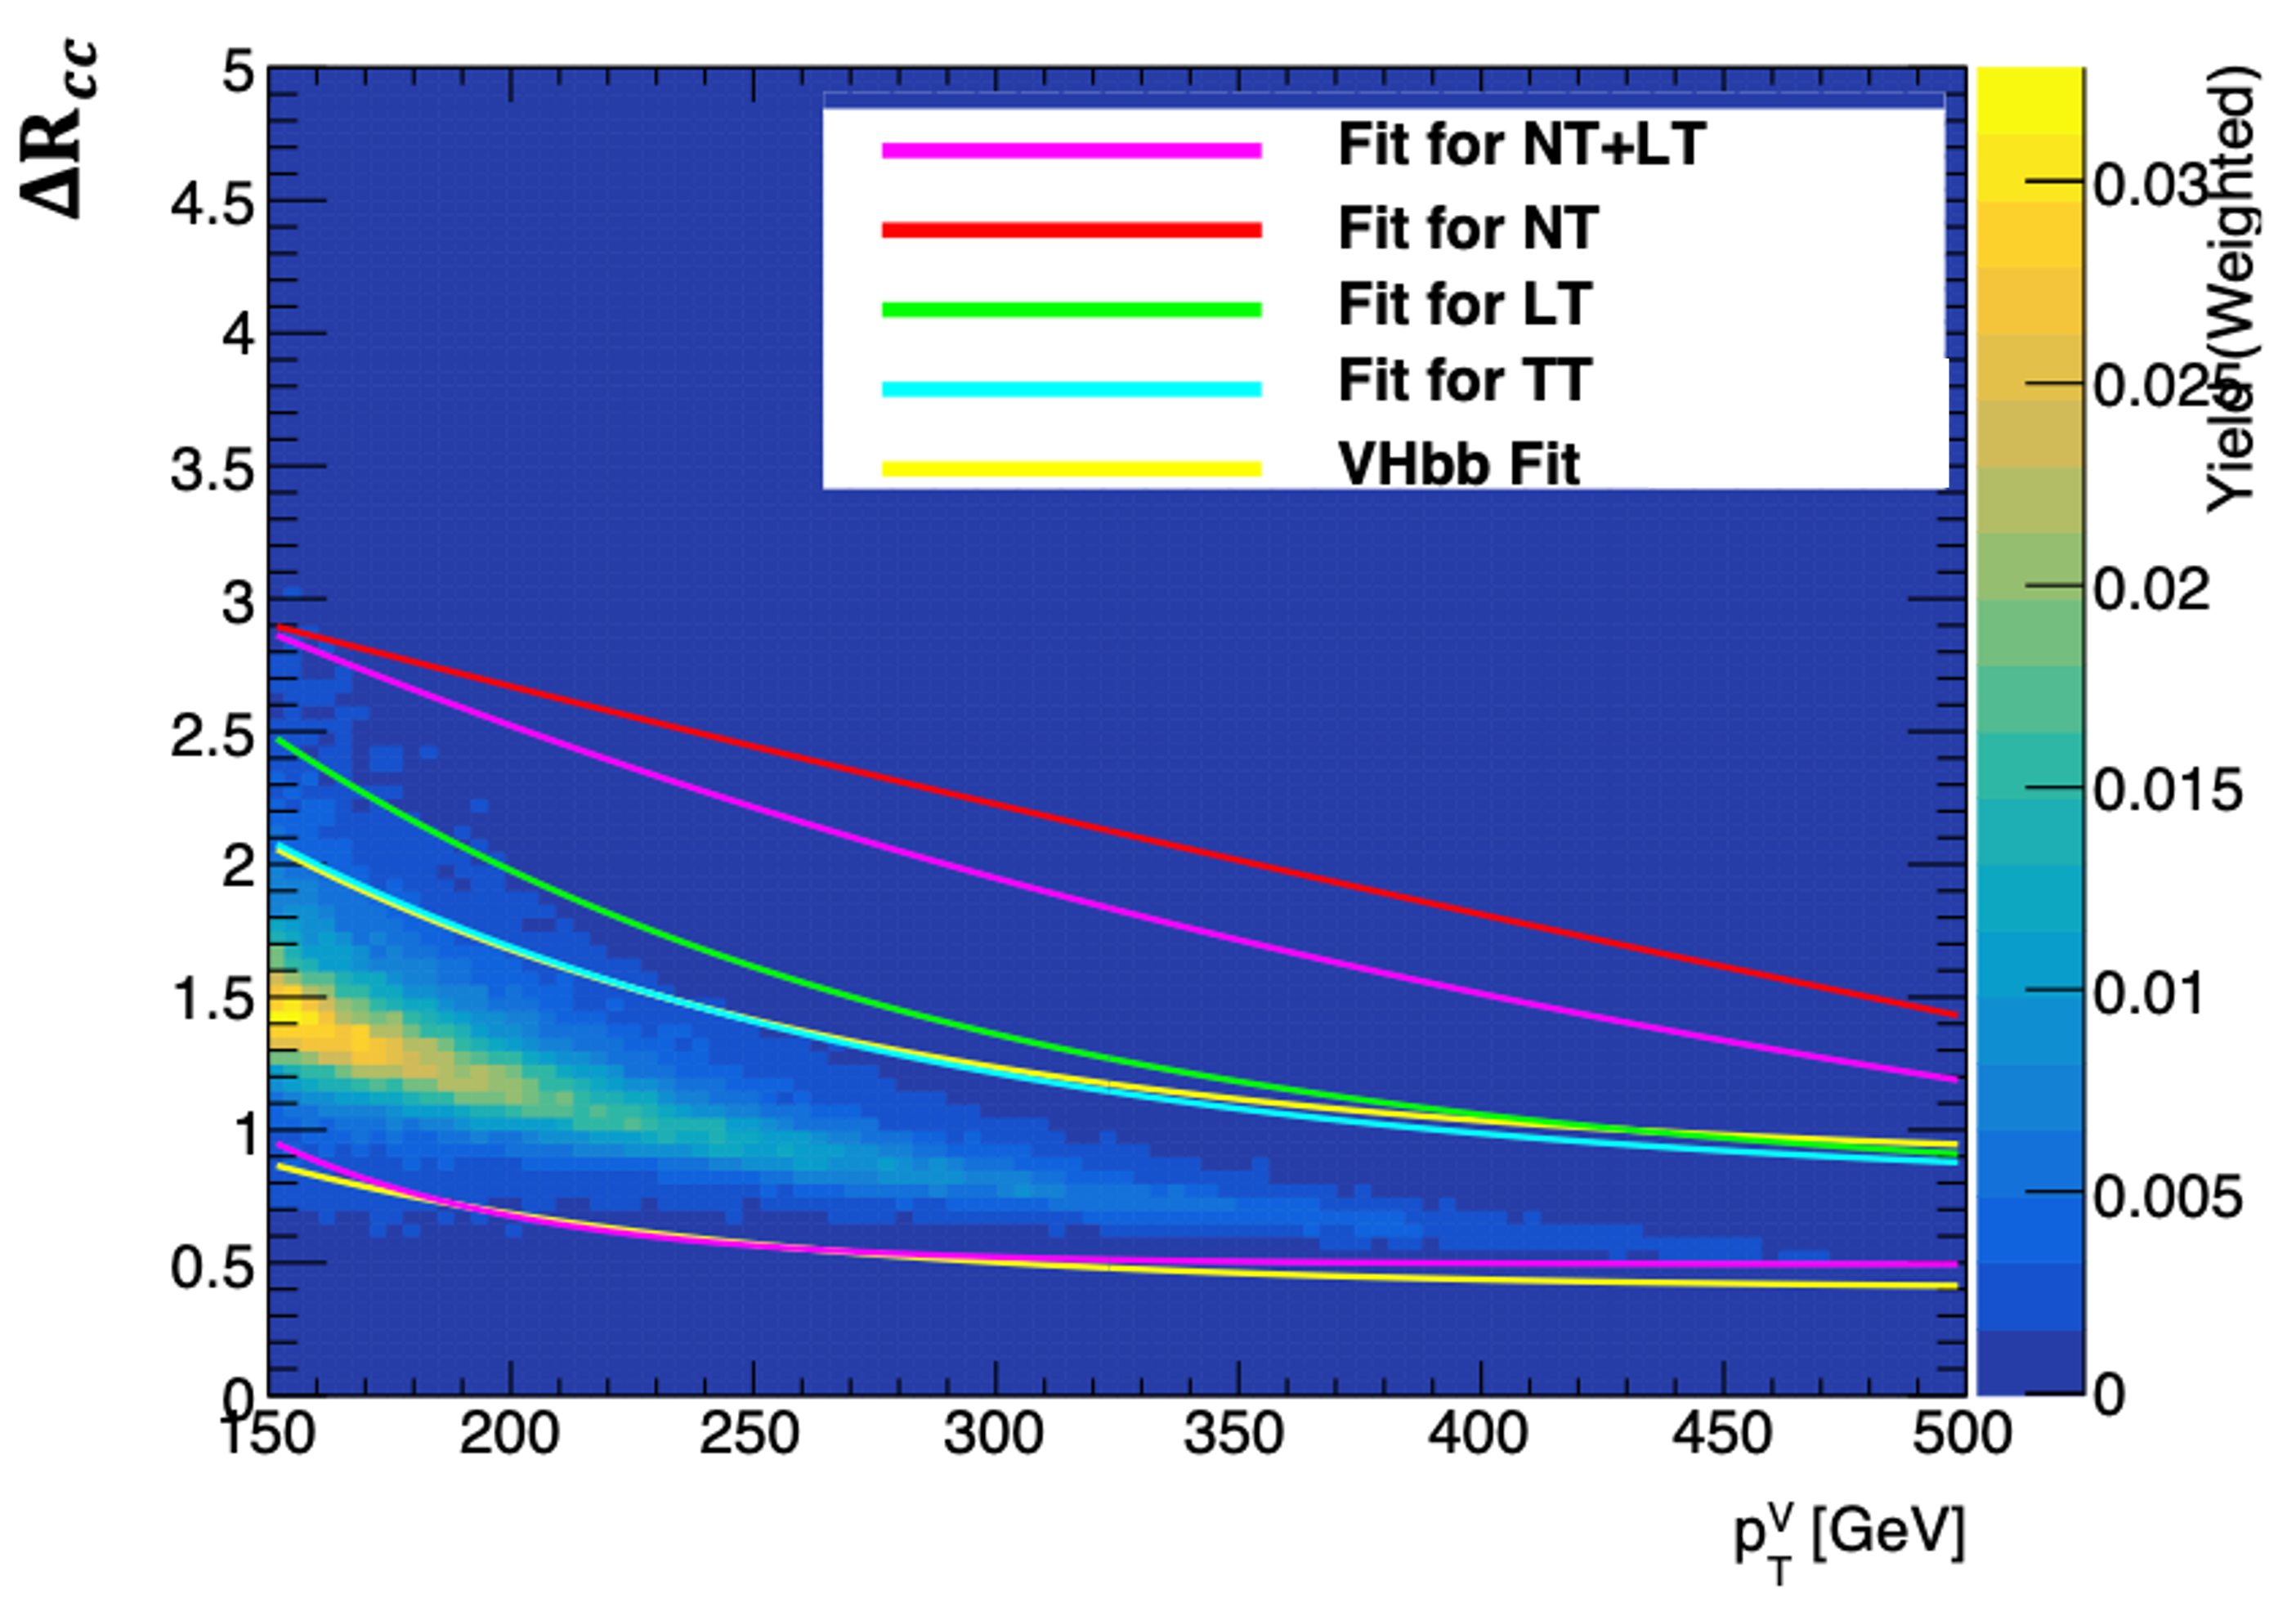
\includegraphics[scale=0.4]{Images/VH/dRccpTV/sr1.png}
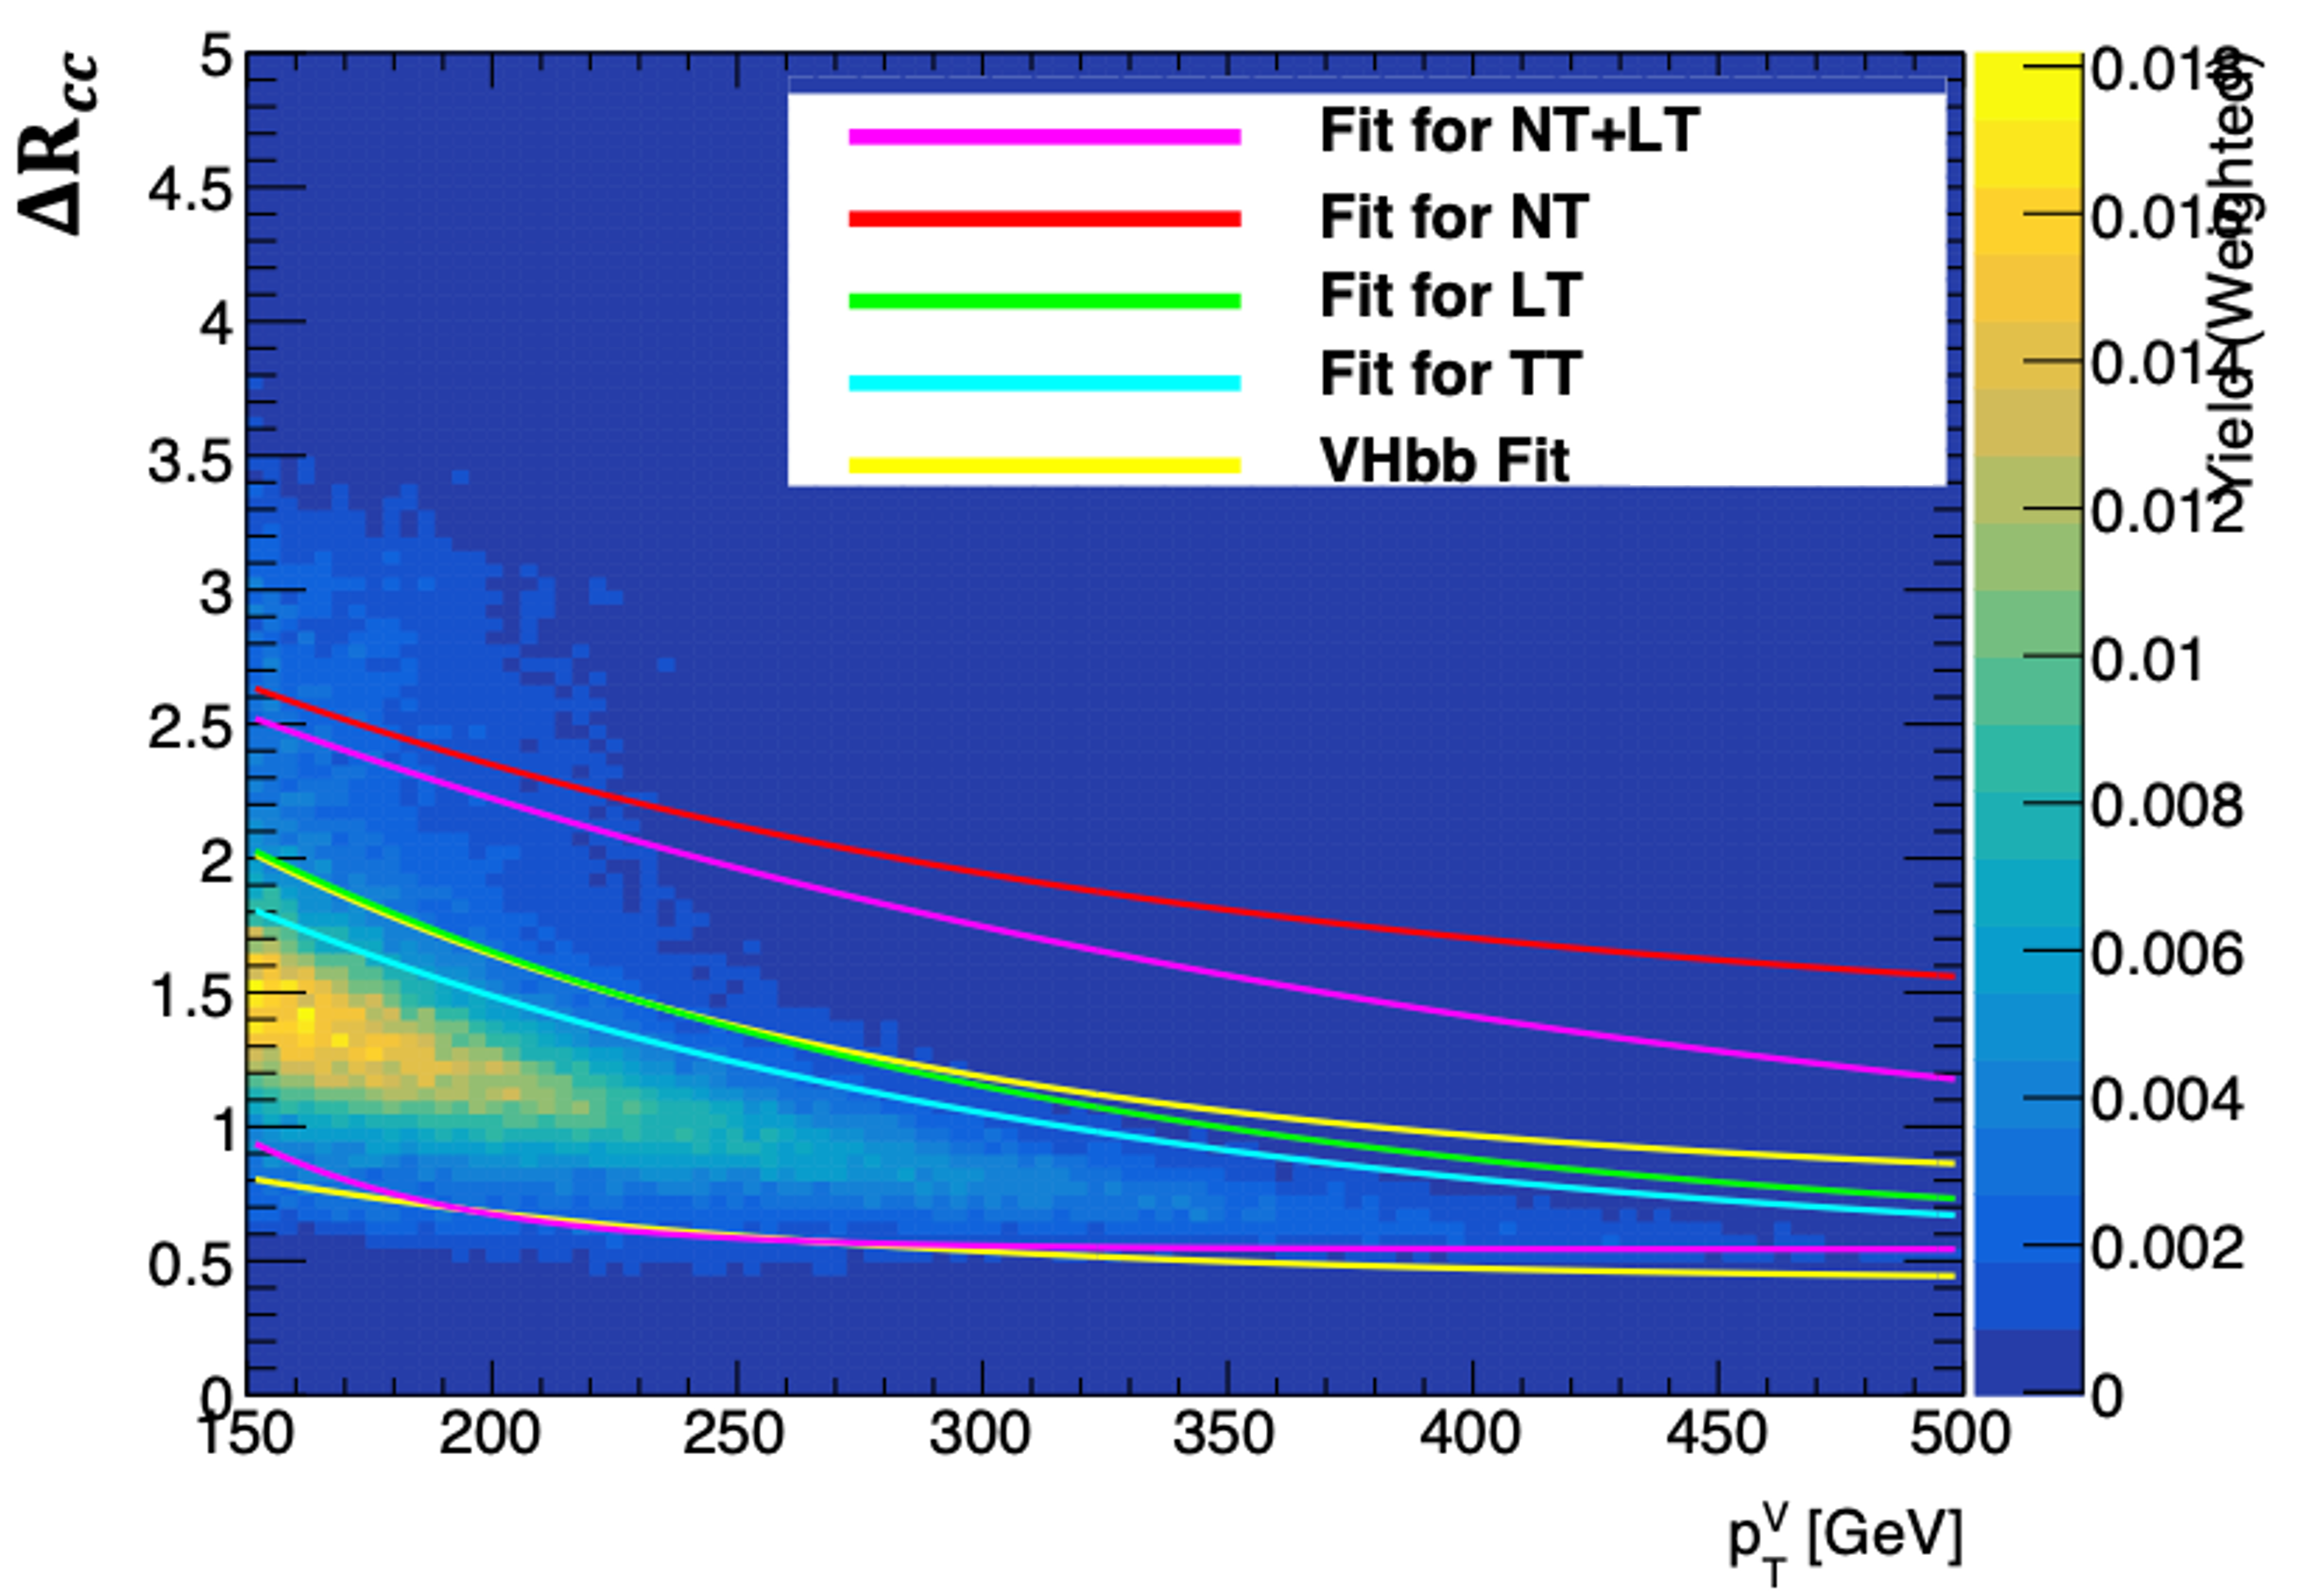
\includegraphics[scale=0.4]{Images/VH/dRccpTV/sr2.png}
\caption{The $p_T^V$-$\Delta R_{c\bar{c}}$ 2D-histograms showing the signal yield of the 1-lepton $VH(H\rightarrow c\bar{c})$, for the 2-jet (left) and 3-jet (right) signal regions. The lines are the results of fitting the $\Delta R_{c\bar{c}}-p_T^V$ cuts for various signal tags, with the yellow curve showing the $VH(H\rightarrow b\bar{b})$ $p_T^V$-$\Delta R_{b\bar{b}}$ cut.} 
\label{fig:drccptvCutsVHcc}
\end{figure}

A summary of the full event categorisation and the regions thus defined at the moment of writing is shown in Figure \ref{fig:ana-strat-det} and a summary of the signal event selection is shown in Table \ref{tbl:VHbbccevSelTable}. As the analysis has not yet concluded, some modifications are still being investigated, such as merging the $LT$- and $TT$-tag regions. An important update to the $VH (H\rightarrow c\bar{c})$ analysis is the introduction of a \textit{Boosted Decision Trees} (BDT) score distribution as discriminant variables instead of the invariant mass of the Higgs candidates jets $m_{c\bar{c}}$. The BDT is trained with kinematic and flavour information about the Higgs candidate jets as well as lepton information and higher-level variables such as angles between the objects, the sum of momenta, and the invariant mass. The algorithm provides a score in the [-1, 1] range corresponding to low or high signal probability and significantly enhances the background-signal separation of the analysis.

\begin{figure}[h!]
\hspace{-2.0cm}
%\center
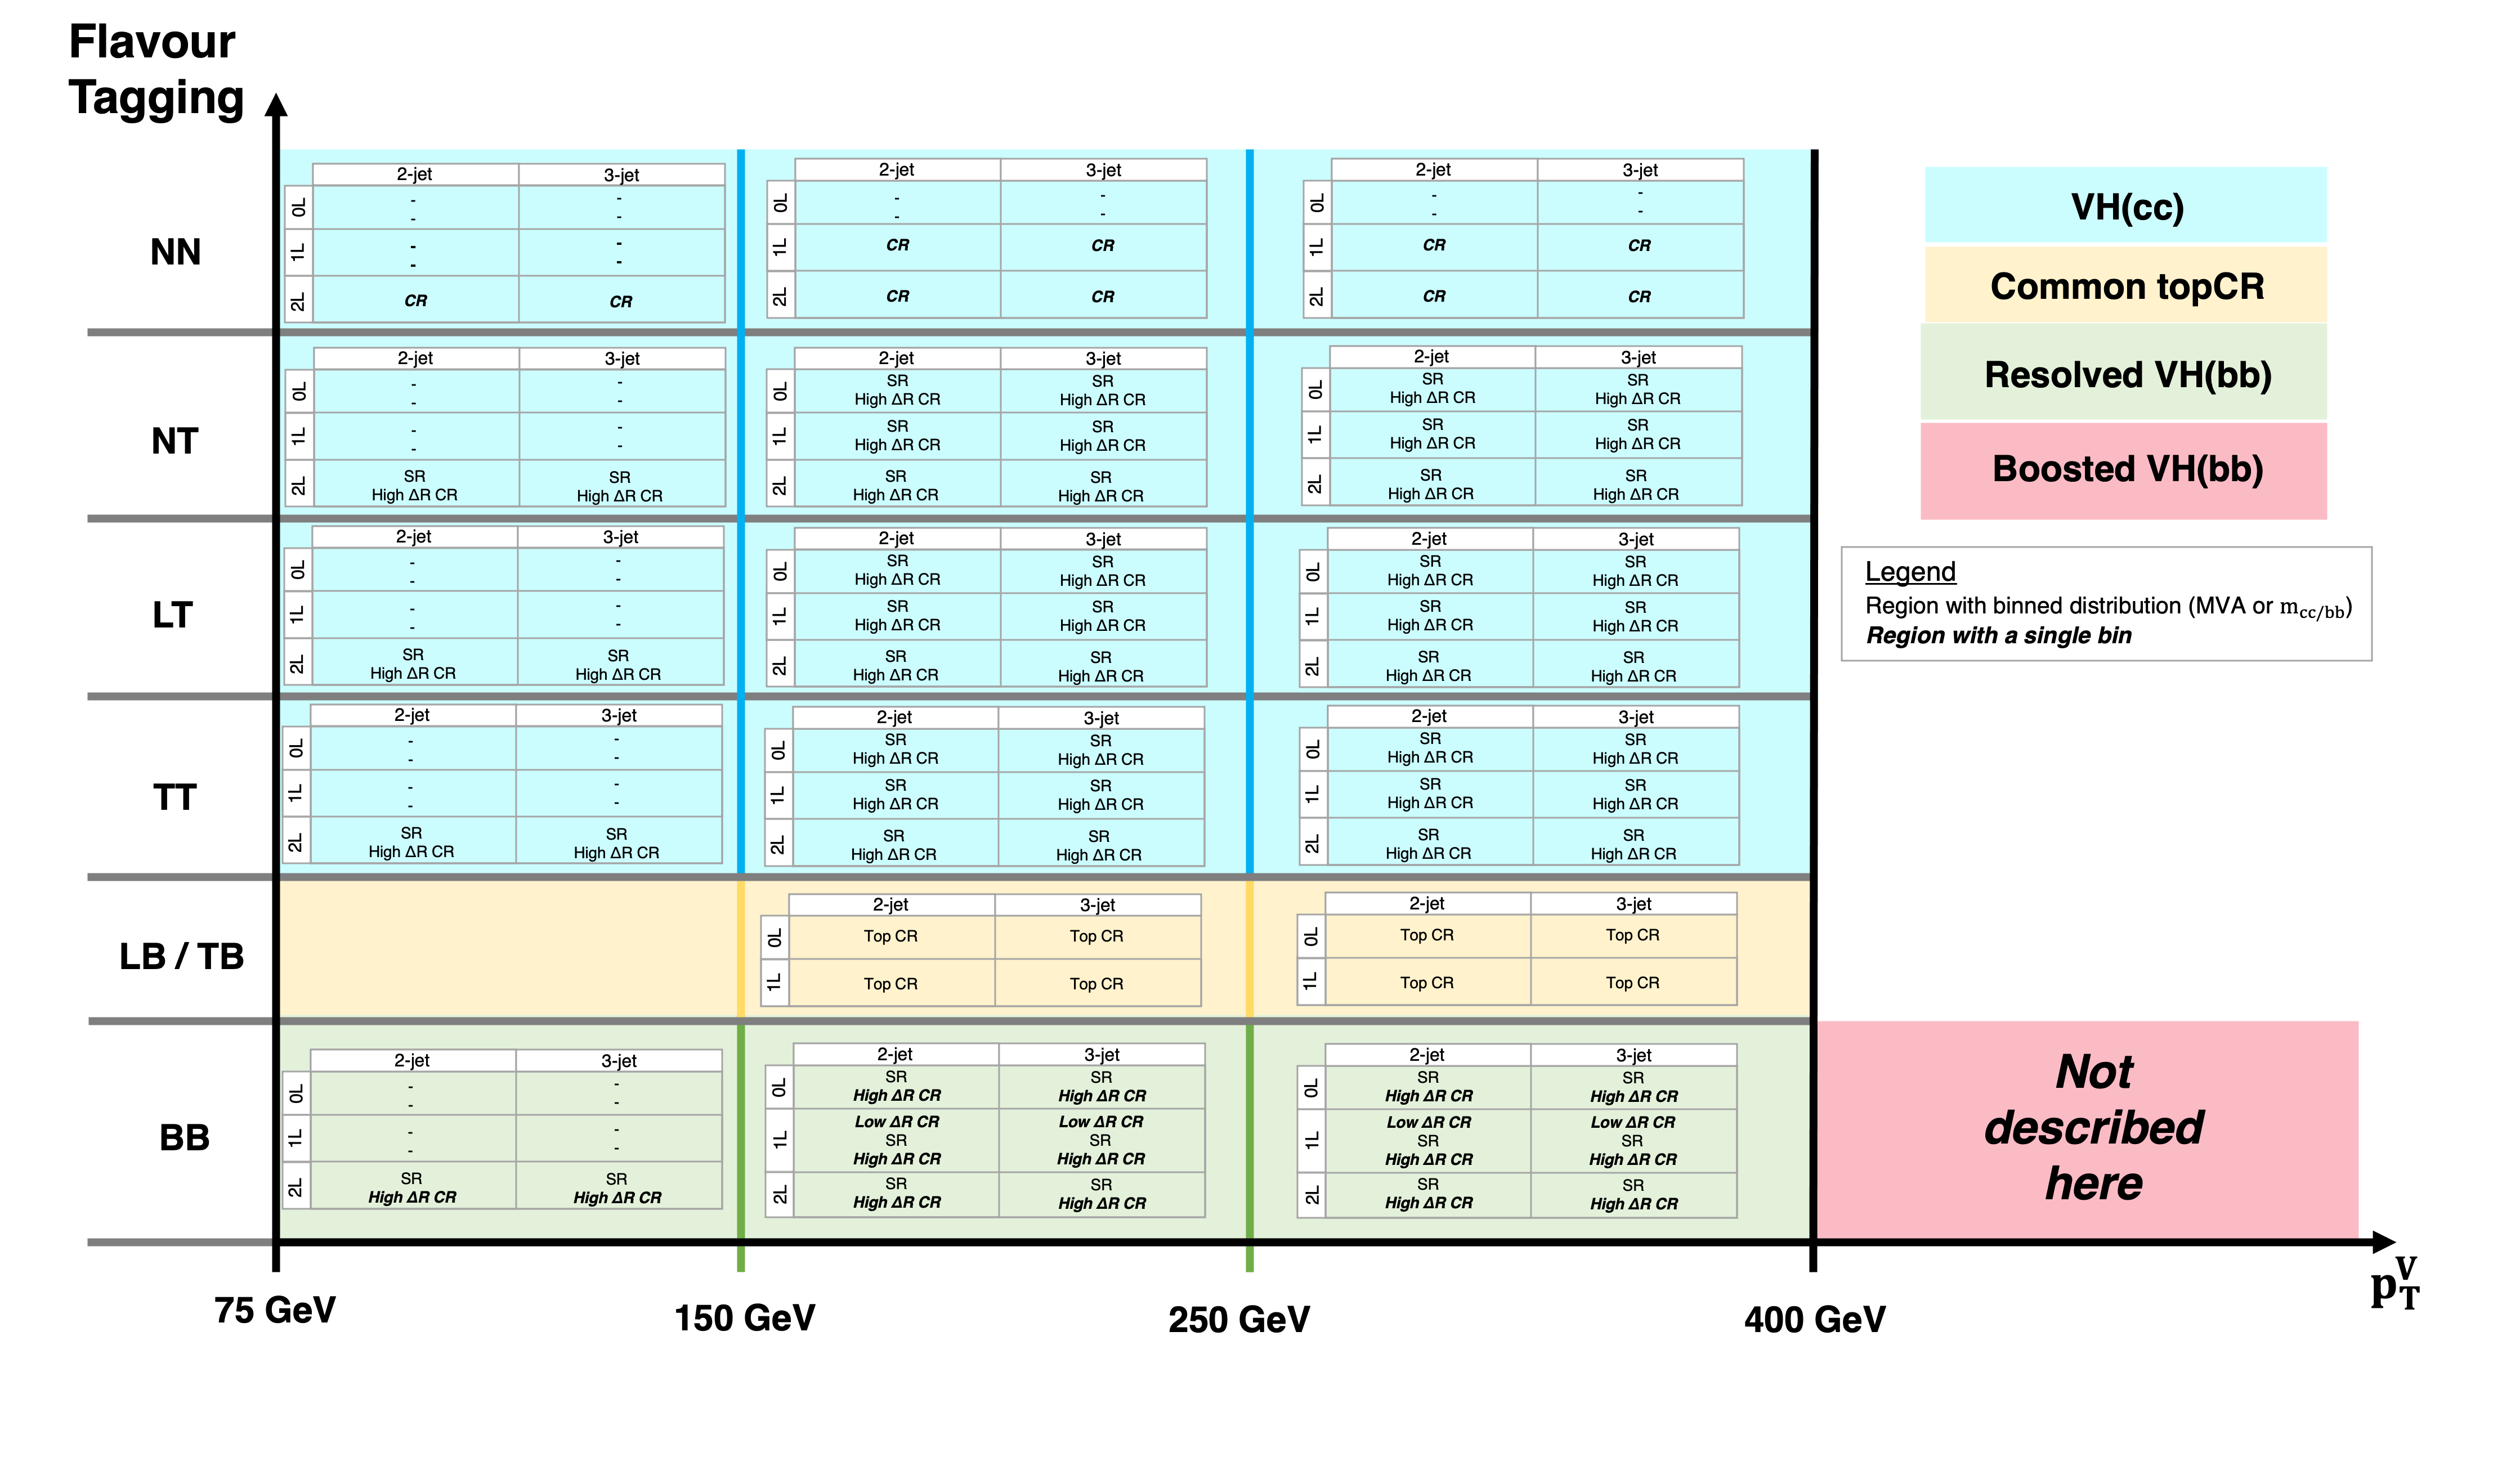
\includegraphics[scale=0.625]{Images/VH/VH_analysis_cat.png}
\caption{The current split of the analysis regions considered in the $VH (H\rightarrow b\bar{b}/c\bar{c})$ Combined Analysis, showing the Signal Region (SR), High and Low $\Delta R$ control region (CR), and the top CR. } 
\label{fig:ana-strat-det}
\end{figure}

%
% From: https://gitlab.cern.ch/atlas-physics-office/HIGG/ANA-HIGG-2020-20/ANA-HIGG-2020-20-INT1/-/blob/master/Tex/TexSubsection/Selection/VHbbccevSelTable.tex
\begin{table}[htbp]
    \begin{center}
    \begin{tabular}{C{6cm}|C{4cm}|C{4cm}}

    \hline \hline
    Analysis regime & $VH(H\rightarrow b\bar{b})$ & $VH(H\rightarrow c\bar{c})$ \\
    \hline \hline
    &\multicolumn{2}{c}{Common Selections}\\
    \hline 
    Jets & \multicolumn{2}{c}{$\geq$ 2 signal jets}  \\
    Candidate jets tagging &  2 B-tags & $\geq1$ T-tag, no B-tag \\
    Leading Higgs candidate jet $p_T$ & \multicolumn{2}{c}{$>$ 45 GeV} \\
    Sub-leading Higgs candidate jet $p_T$ & \multicolumn{2}{c}{$>$ 20 GeV} \\
    Non-H candidate jet $p_T$ & \multicolumn{2}{c}{$>$ 30 GeV} \\
    $\Delta R$(jet1, jet2)  & \multicolumn{2}{c}{Cuts applied (see above)} \\

    \hline \hline
    &\multicolumn{2}{c}{0 Lepton} \\
    \hline
    Trigger & \multicolumn{2}{c}{$E_T^{\textrm{miss}}$ triggers} \\
    Jets & \multicolumn{2}{c}{$\leq$ 3  jets}  \\
    Non-H candidate jets tagging & no T-tag & - \\
    Leptons & \multicolumn{2}{c}{0 $VH$-loose leptons} \\
    $E_T^{\textrm{miss}}$ & \multicolumn{2}{c}{$>$ 150~GeV}  \\
    $E_{T, trk}^{\textrm{miss}}$  & - & $>$ 30~GeV \\
    $\sum_i p_T^{\textrm{jet}_i}$ & \multicolumn{2}{c}{$>$ 120 (2 jets), $>$150 GeV (3 jets)}  \\
    $| \textrm{min}\Delta \phi (E_T^{\textrm{miss}}, \textrm{jet})|$& \multicolumn{2}{c}{$>20\ensuremath{^\circ}$ (2 jets), $> 30\ensuremath{^\circ}$(3 jets)} \\
    $|\Delta\phi(E_T^{\textrm{miss}}, H)|$ & \multicolumn{2}{c}{$> 120\ensuremath{^\circ}$} \\
    $|\Delta\phi(\textrm{jet1, jet2})|$ & \multicolumn{2}{c}{$< 140\ensuremath{^\circ}$} \\
    $|\Delta\phi(E_T^{\textrm{miss}},E_{T, trk}^{\textrm{miss}})|$ & \multicolumn{2}{c}{$< 90\ensuremath{^\circ}$} \\
    $p_T^V$ regions & \multicolumn{2}{c}{[150, 250]~GeV, [250, 400]~GeV}  \\


    \hline\hline
    &\multicolumn{2}{c}{1 Lepton} \\
    \hline
    Trigger &  \multicolumn{2}{c}{$e$ channel: single electron trigger} \\
            & \multicolumn{2}{c}{$\mu$ channel: single muon trigger ($p_T^V <$ 150 GeV)} \\
            & \multicolumn{2}{c}{and  $E_T^{\textrm{miss}}$ triggers (above)} \\
    Jets & \multicolumn{2}{c}{$\leq$ 3  jets}  \\
    Candidate jets tagging & no T-tag & - \\
    hadronic $\tau$-veto & \multicolumn{2}{c}{no hadronic $\tau$} \\
    Leptons & \multicolumn{2}{c}{1 $WH$-signal lepton} \\
            &  \multicolumn{2}{c}{$>1$~$VH$-loose lepton veto} \\
    $E_T^{\textrm{miss}}$   & \multicolumn{2}{c}{$>$ 30~GeV ($e$ channel)} \\
    $p_T^V$ regions & \multicolumn{2}{c}{[150, 250]~GeV, [250, 400]~GeV}  \\


    \hline\hline
    & \multicolumn{2}{c}{2 Lepton}\\
    \hline
    Trigger &  \multicolumn{2}{c}{as for 1L but the $p_T^V$ limit for $\mu$ is 250 GeV}\\
    Leptons & \multicolumn{2}{c}{2 $VH$-loose leptons} \\
            & \multicolumn{2}{c}{($\ge$ 1 $ZH$-signal lepton)} \\
            & \multicolumn{2}{c}{Same flavour,}\\
            & \multicolumn{2}{c}{Opposite-charge for $\mu\mu$} \\
    $m_{ll}$   & \multicolumn{2}{c}{81 $<$ $m_{ll}$ $<$ 101~GeV} \\
    %$E_T^{\textrm{miss}}$ significance (cut-based)  & \multicolumn{2}{c}{E_T^{\textrm{miss}}$/\sqrt{\textrm{HT}} < 3.5\sqrt{GeV}$} \\
    $p_T^V$ regions & \multicolumn{2}{c}{[75,150], [150, 250], [250, 400]~GeV}  \\
    \hline\hline

    \end{tabular}
    \caption{Summary of the signal event selection in the 0-, 1- and 2-lepton channels (adapted from the internal note). Variables not presented in the text: $E_{T, trk}^{\textrm{miss}}$ is the missing transverse momentum calculated from the negative vector sum of the transverse momenta of tracks reconstructed in the inner detector and identified as originating from the primary vertex and $m_{ll}$ is the invariant mass of the di-lepton pair. }
    \label{tbl:VHbbccevSelTable}
    \end{center}
    \end{table}
%

\subsubsection{Top Control Region}
The top control region (topCR) is used to constrain the rather significant top background that peaks at signal-like values of the discriminant variables. Indeed, when the candidate jets selected correspond to the $b$- and $c$-jet from a $t\bar{t}$ decay, the invariant mass of the pair peaks at 120 GeV, exactly the region of interest for a Higgs decay search. The topCR is defined by requiring at least one $c$-tagged jet in combination with at least one $b$-tagged jet using the \textit{AllSignal} strategy, as previously described. This tagging requirement renders it orthogonal to the signal region of the analysis and targets the decay topology of the different top processes: 
\begin{itemize}
\item Semi-leptonic $t\bar{t}$ decay: both $t$ follow the usual decay chain  $t \rightarrow b$ + $W$, with one of the $W$ decaying leptonically and the other one to a pair of quarks. Some events from this process can enter the signal region when some of the quarks are $c$-tagged or if the $b$-jets are mis-tagged or flew out of the detector acceptance. Requiring the combination of a $b$-tag and a $c$-tag effectively selects this process, the $b$ coming from the direct $t$ decay and the $c$ from a subsequent $W$ decay. 
\item Single top $t$-quark: predominantly the $Wt$ process $W$ $t \rightarrow W$ +  $b$ + $W$, with one $W$ decaying leptonically and the other hadronically. Some of these background events can enter the signal region if the $b$- is missed and if a jet is $c$-tagged, from the extra $W$ or if the $b$-jet is mis-tagged. Events from the single-top $t$- and $s$-channel of the process $t \rightarrow b$ + $W$ bring a smaller contribution, as the $c$-tagged jet must come from \textit{Initial State Radiation} (ISR) or \textit{Final State Radiation} (FSR) if the $b$ is not mis-tagged. Single-top is a minor background in 0L and 1L, with the main component being the production of $Wt$ pairs. The $t$-channel and $s$-channel contribute less than 1\% of the total background.
\end{itemize}

Of the two processes, the $t\bar{t}$ is therefore the most important one and a main background in the 0L and 1L channels. Due to their similarities, the $t\bar{t}$ and $Wt$ processes are considered as a single \textit{top} background in the analysis. In 2L, because this top background is small, no flavour-based topCRs are introduced and a different strategy is employed where the top is directly constrained in a pure top-$e\mu$ control region defined by requiring two charged leptons of different flavours. For the 0L and 1L channels, the expected top background normalisation and its kinematic distributions, as given by the MC simulation, are adjusted using data in the topCRs; this is extrapolated to the signal regions under consideration of extrapolation effects (and corresponding extrapolation uncertainties) that account for differences between the topCRs and SRs. \\

The combined top background is separated into different components, depending on the true flavour of the two candidate jets, that can be combined during the statistical analysis. These are:
\begin{itemize}
\item top($bb$): in this case, the two $b$-jets produced during the $t\bar{t}$ decay are selected. This is a small component in the signal regions of the $VH(H\rightarrow c\bar{c})$ analysis, due to the 70\% efficiency WP for $b$-tagging and the low mis-tag rate for $b$-jets in $c$-tagging. Naturally, in $VH(H\rightarrow b\bar{b})$ it is the leading contribution. Due to the origin of the candidate jets, a large $\Delta R_{b\bar{b}}$ is expected between the two $b$-jets so this component is most effectively constrained by the High $\Delta R$ CR. 
\item top($bc$): where the $b$ is from a $t$ decay and the $c$ from a subsequent $W$ hadronic decay (or from ISR/FSR though this is less likely). Given the definition of the topCR, this is the dominating component in that region and the most important to constrain in the signal regions of the $VH(H\rightarrow b\bar{b}/c\bar{c})$ analyses due to its signal-like kinematics. 
\item top($bl$): where $l$ stands for anything not $b$ nor $c$ (light jets predominantly but also some mis-tagged hadronic $\tau$). This component is similar to the top($bc$) as it also consists of a $b$ + a jet from the $W$ and can end up in the SRs and topCRs due to mis-tags.
\item top($lq$): where $l$ is as above and $q$ can be any sort of jet except a $b$. This is a small component that mostly accumulates in the background-like part of the BDT score distribution. It is not constrained in the high $\Delta R$ regions nor the topCRs.
\end{itemize}
The signal region distributions in the 1L channel in the $p_T^V$ range $[150, 250]$ GeV are displayed in Figure \ref{fig:SRslowptv}. While the top is not the dominant background, except in the tighter tagged TT 3-jet region, its relative contribution to the background composition increases at signal-like values of the discriminant, as shown in Figure \ref{fig:topContentSR}. \\

\begin{figure}[h!]
%\hspace{-2.0cm}
\center
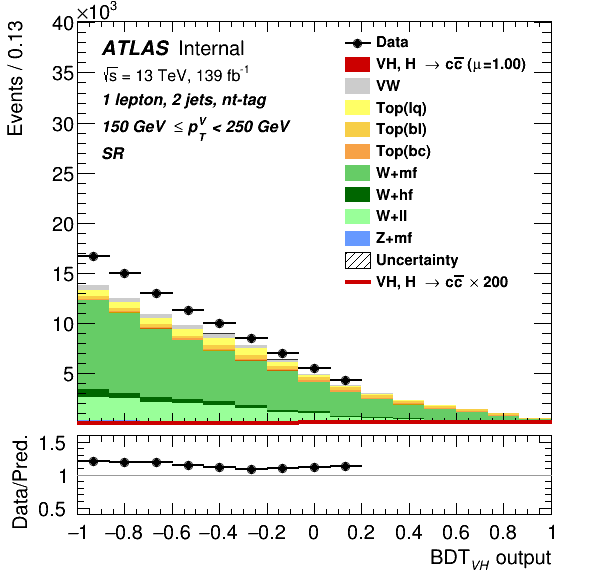
\includegraphics[scale=0.2753]{Images/VH/SRsandTopCRs/Region_distmva_DSR_BMax250_L1_Y6051_TTypent_T1_J2_BMin150_Prefit.png}
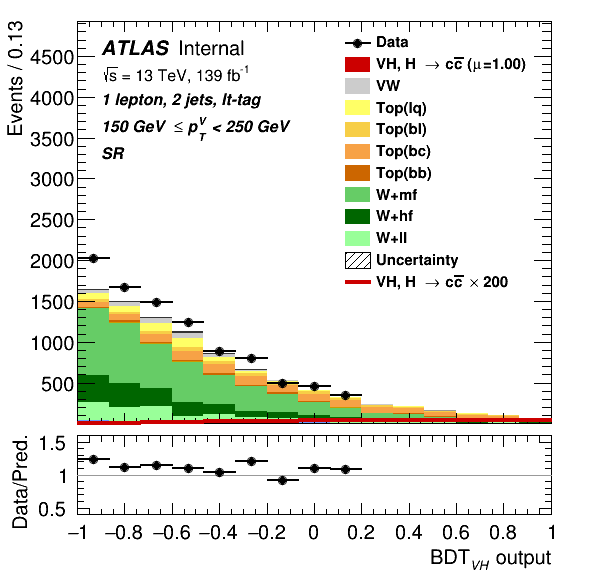
\includegraphics[scale=0.2753]{Images/VH/SRsandTopCRs/Region_distmva_DSR_BMax250_L1_Y6051_TTypelt_T2_J2_BMin150_Prefit.png}
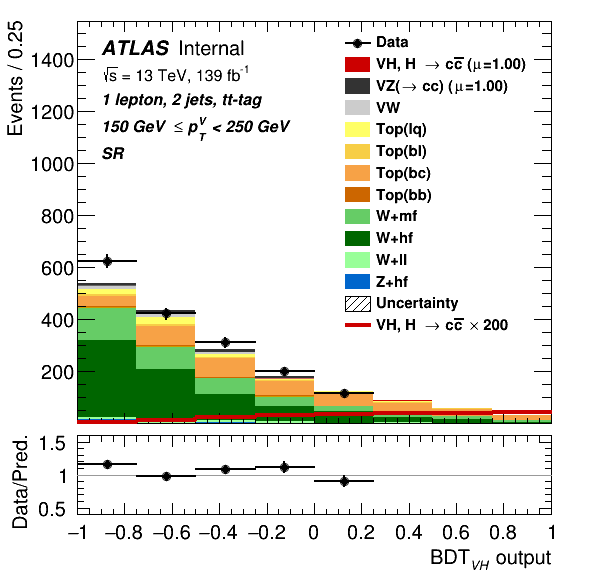
\includegraphics[scale=0.2753]{Images/VH/SRsandTopCRs/Region_distmva_DSR_BMax250_L1_Y6051_TTypett_T2_J2_BMin150_Prefit.png}\\
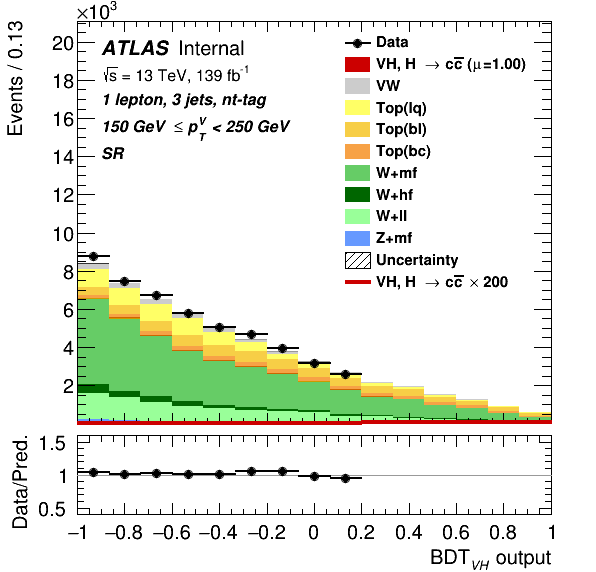
\includegraphics[scale=0.2753]{Images/VH/SRsandTopCRs/Region_distmva_DSR_BMax250_L1_Y6051_TTypent_T1_J3_BMin150_Prefit.png}
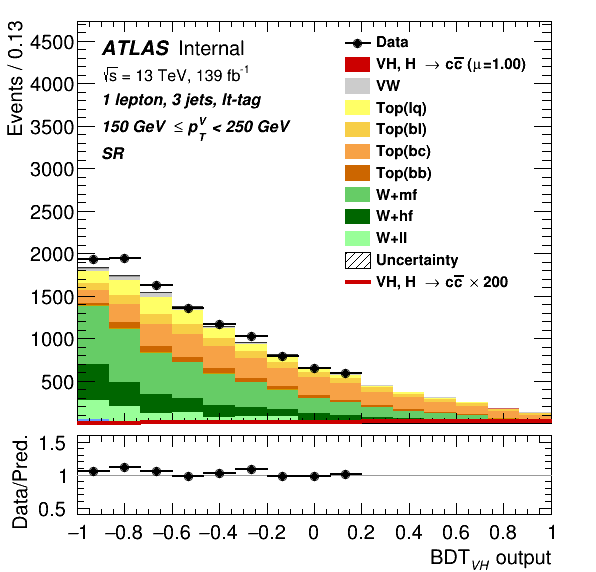
\includegraphics[scale=0.2753]{Images/VH/SRsandTopCRs/Region_distmva_DSR_BMax250_L1_Y6051_TTypelt_T2_J3_BMin150_Prefit.png}
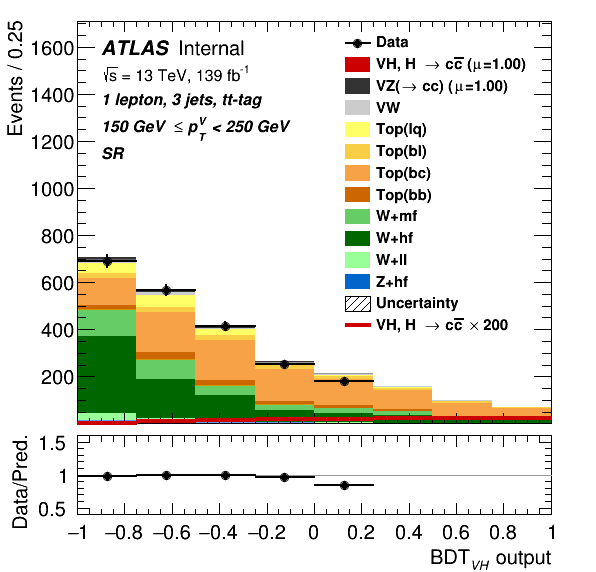
\includegraphics[scale=0.2753]{Images/VH/SRsandTopCRs/Region_distmva_DSR_BMax250_L1_Y6051_TTypett_T2_J3_BMin150_Prefit.png}
\caption{The 1L signal regions BDT distributions in the low [150-250] $p_T^V$ range. Left: NT; centre: LT; right: TT. Top: 2 jets; bottom: 3 jets.} 
\label{fig:SRslowptv}
\end{figure}

The components contributing the most in the $VH(H\rightarrow c\bar{c})$ side of the analysis are the top($bc$) and top($bl$), due to the tagging requirement. There is very little top($bb$) thanks to the good performance of the tagger. Top($lq$) is mostly found in the looser tag regions (NT, LT) and not where the signal peaks. Figure \ref{fig:topCRslowptv} displays the new top control regions proposed in this work: as expected, the bulk of the distributions is made of top background, centred around the expected Higgs mass. The philosophy behind the proposed new design leverages the pseudo-continuous tagging to select the highest $p_T$ $b$-tagged and $c$-tagged jets as Higgs candidates. Thus, BL and BT regions are defined depending on whether the highest $p_T$ $c$-tagged jet is loose- or tight-tagged. The regions are further split in the number of jets and the same definition is used in the 0L channel. The full tag compositions of each region are as follows:

\begin{itemize}
\item 2-jet: \quad BL: $BL$;  \quad BT: $BT$
\item 3-jet:  \quad BL: $BLN$, $BLL$;  \quad BT: $BTN$, $BTL$, $BTT$, and $BBT$
\end{itemize}
In the \textit{AllSignal} strategy, the Higgs candidates in the topCR are always the highest $p_T$ $b$- and $c$-tagged jets. This selection was observed to make the top control region distributions more closely match the distributions in the signal regions. \\

\begin{figure}[h!]
\vspace{0.5cm}
\center
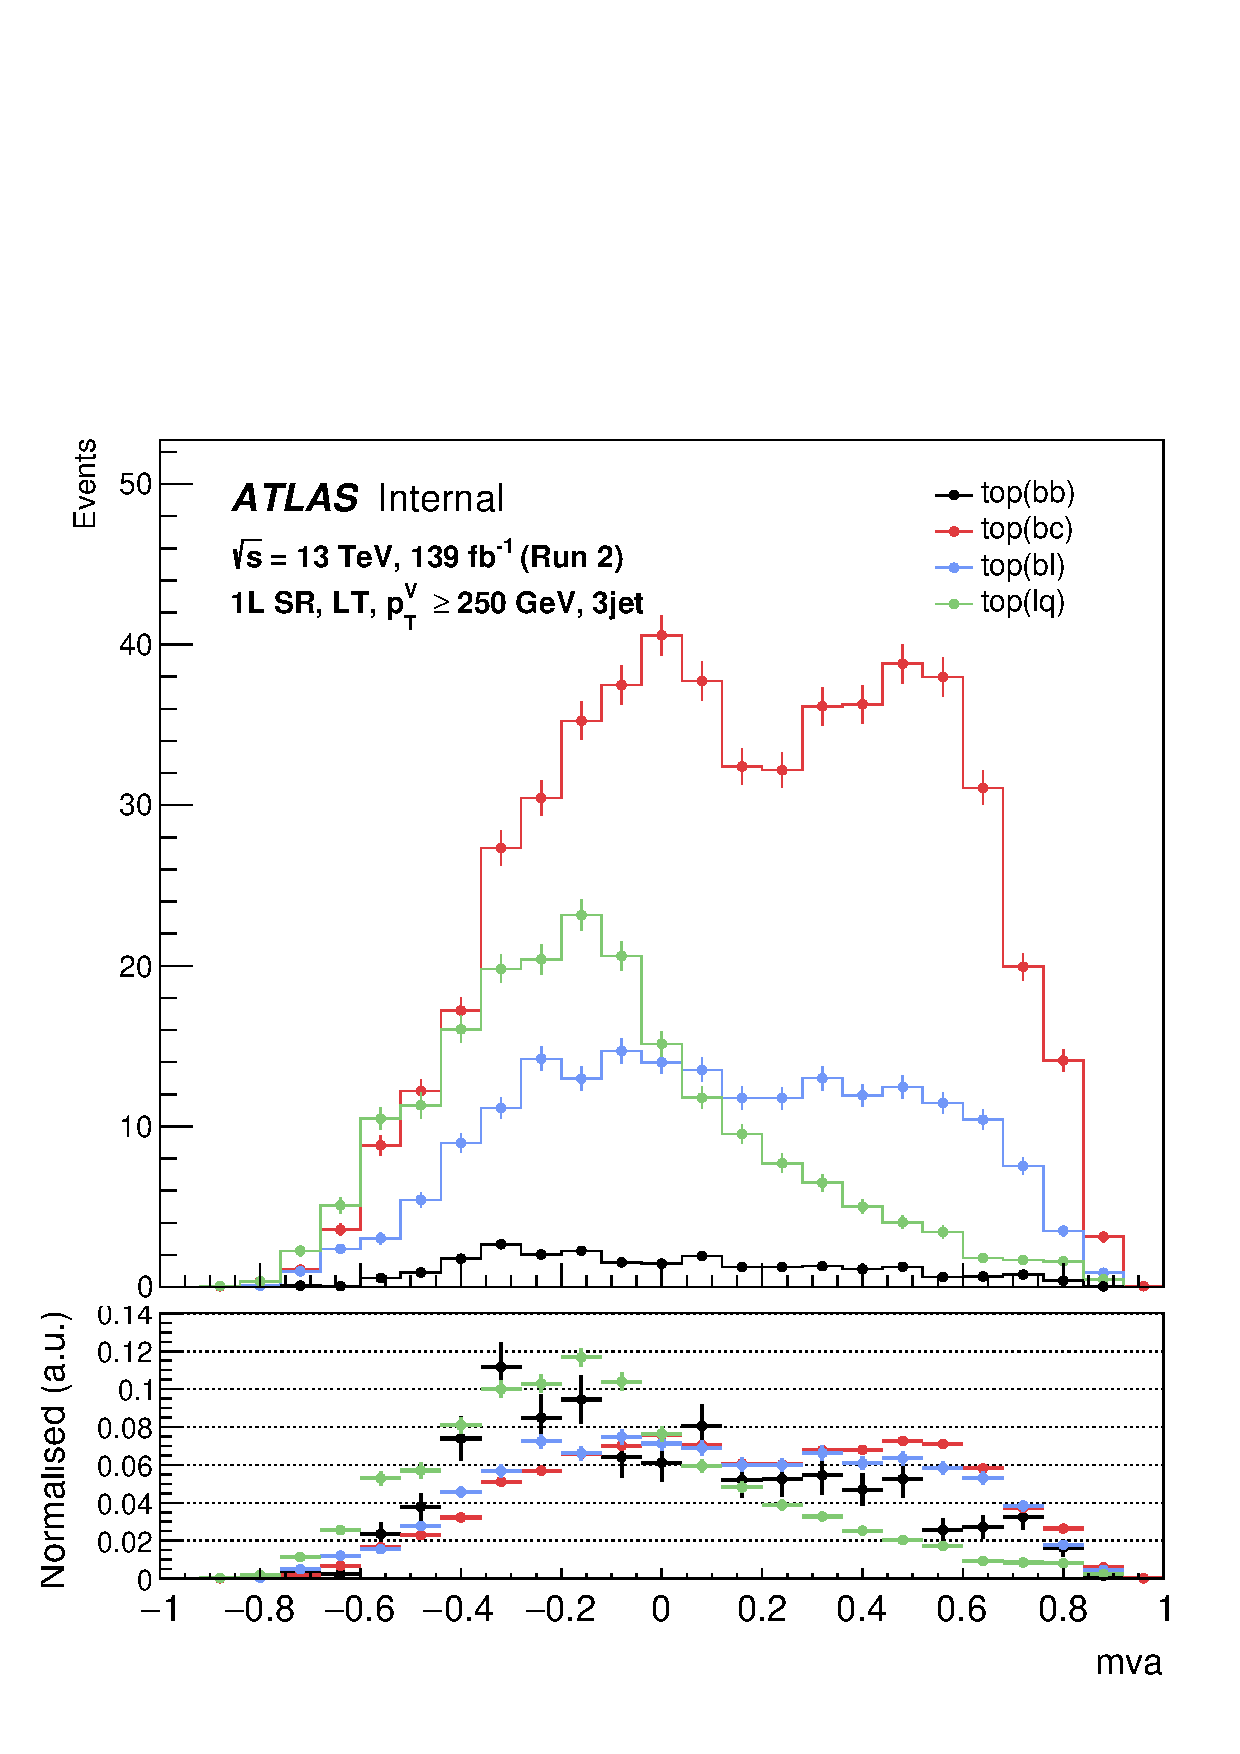
\includegraphics[scale=0.4]{Images/VH/top/OneLepton_top_2lttag3jet_SR_250ptv_mva.pdf}
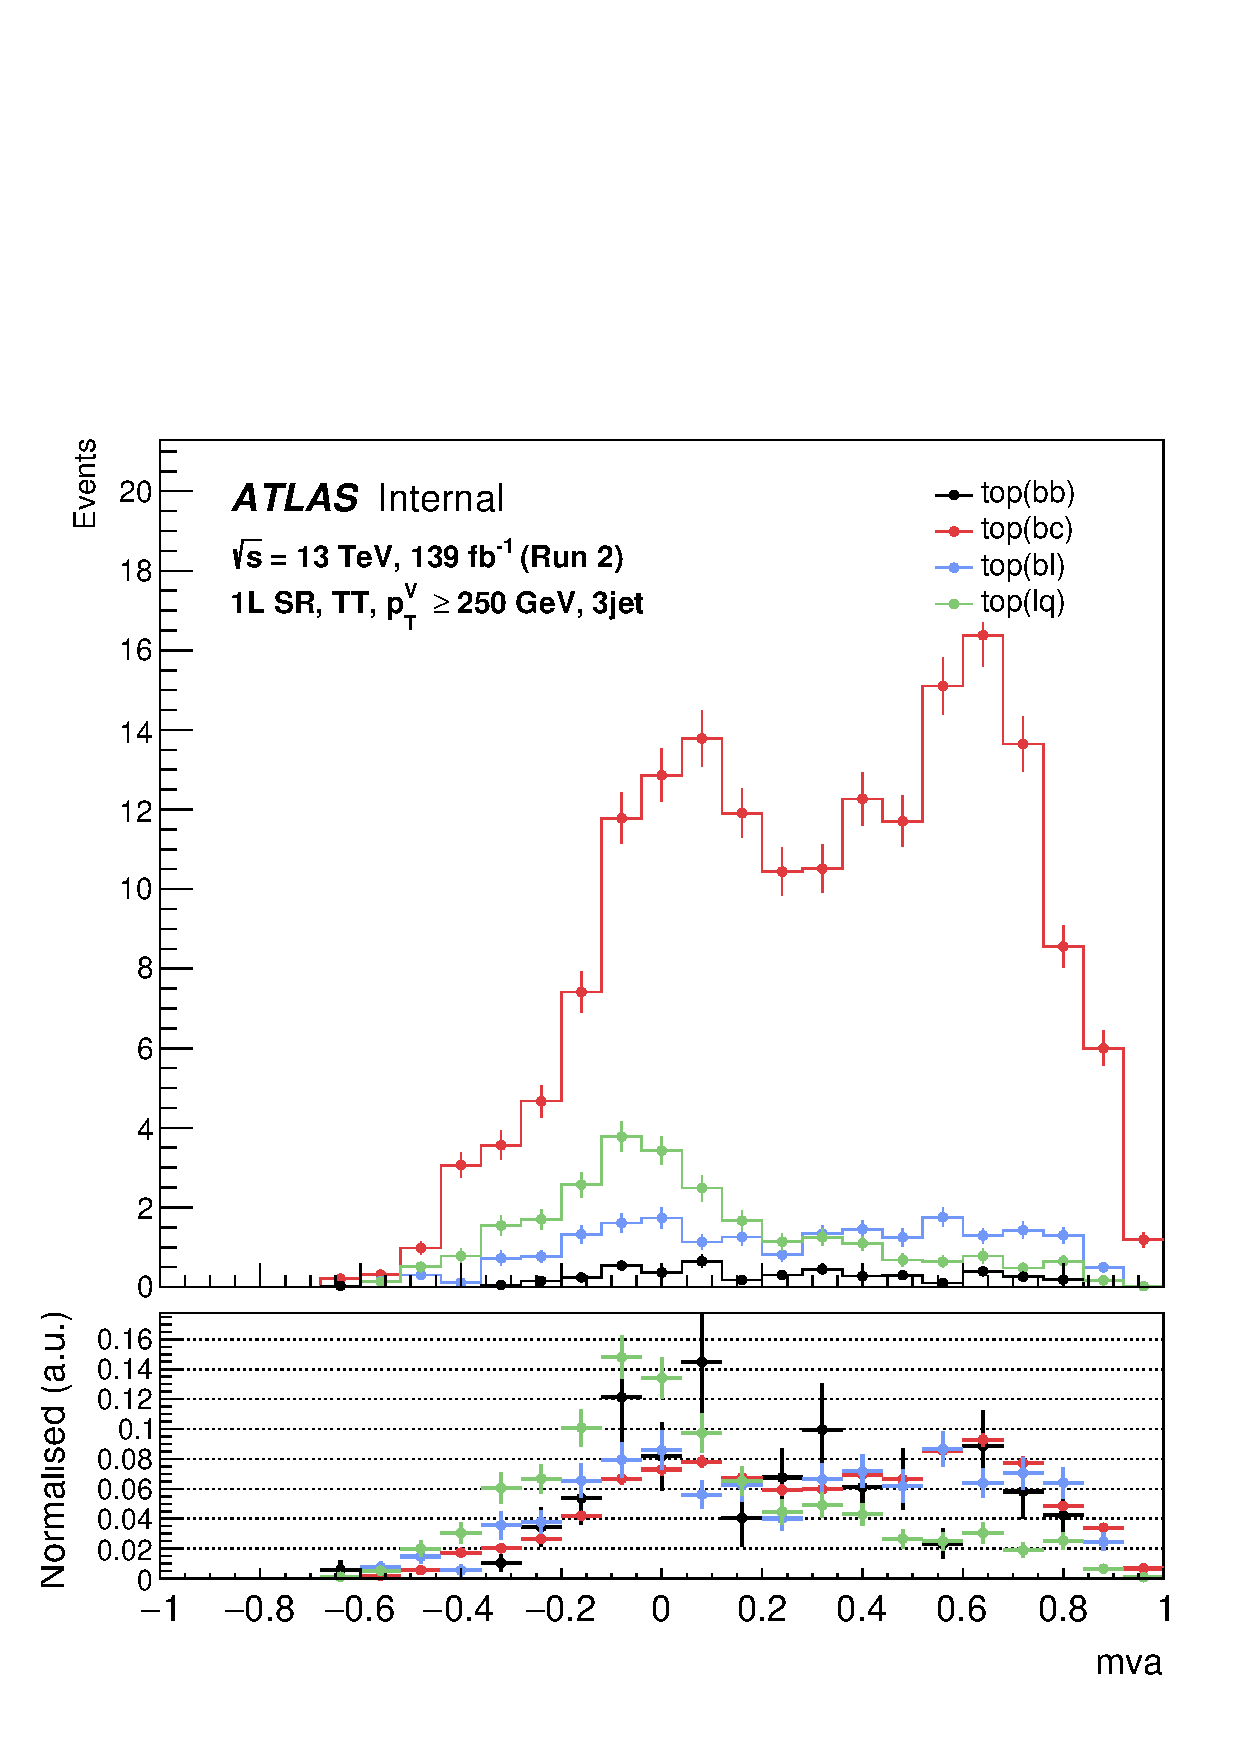
\includegraphics[scale=0.4]{Images/VH/top/OneLepton_top_2tttag3jet_SR_250ptv_mva.pdf}
\caption{Top components in the 1L 3 jets signal regions BDT distributions in the $\geq$ 250 GeV $p_T^V$ range. Left: LT; right: TT.}
\label{fig:topContentSR}
\end{figure}

\begin{figure}[h!]
%\hspace{-2.0cm}
\center
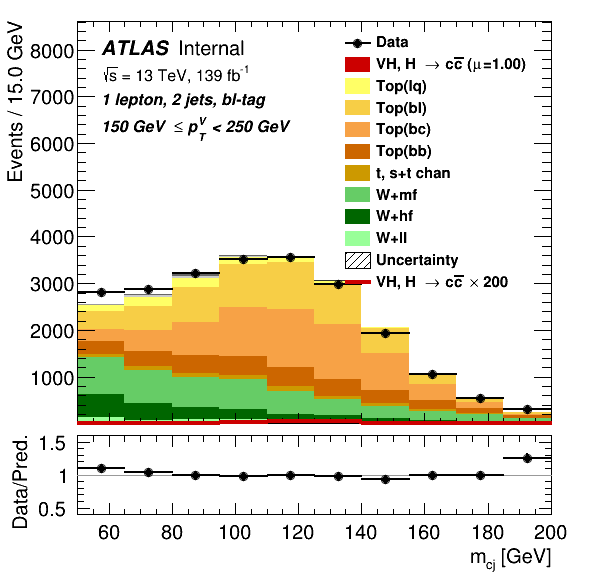
\includegraphics[scale=0.2]{Images/VH/SRsandTopCRs/Region_distmBB_DtopCRBL_BMax250_L1_Y6051_TTypebl_T1_J2_BMin150_Prefit.png}
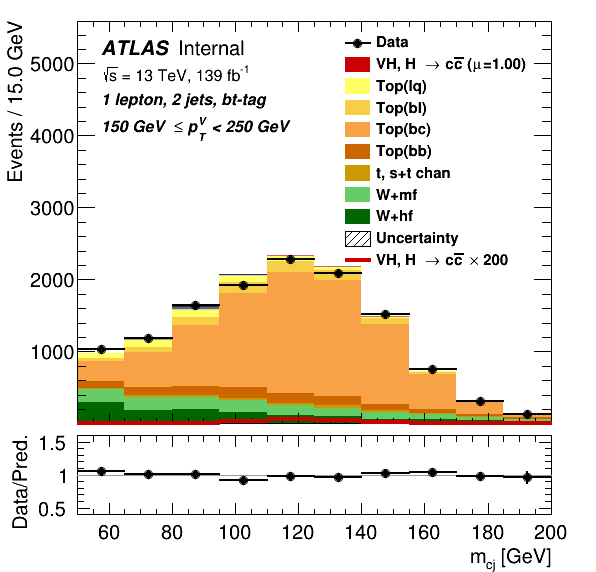
\includegraphics[scale=0.2]{Images/VH/SRsandTopCRs/Region_distmBB_DtopCRBC_BMax250_L1_Y6051_TTypebt_T1_J2_BMin150_Prefit.png}
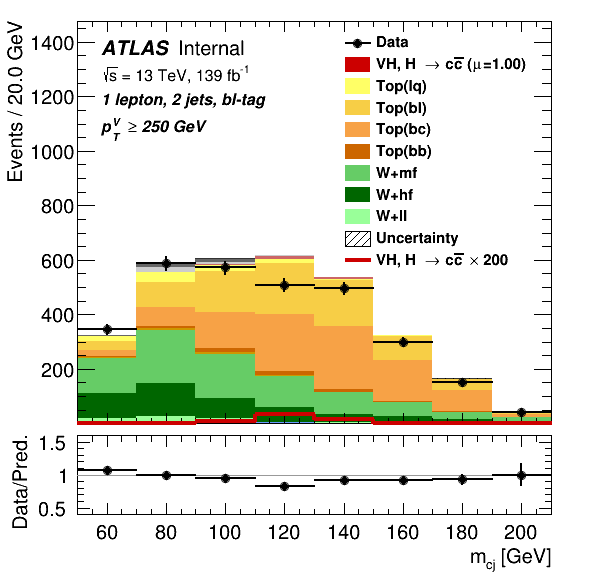
\includegraphics[scale=0.2]{Images/VH/SRsandTopCRs/Region_distmBB_DtopCRBL_L1_Y6051_TTypebl_T1_J2_BMin250_Prefit.png}
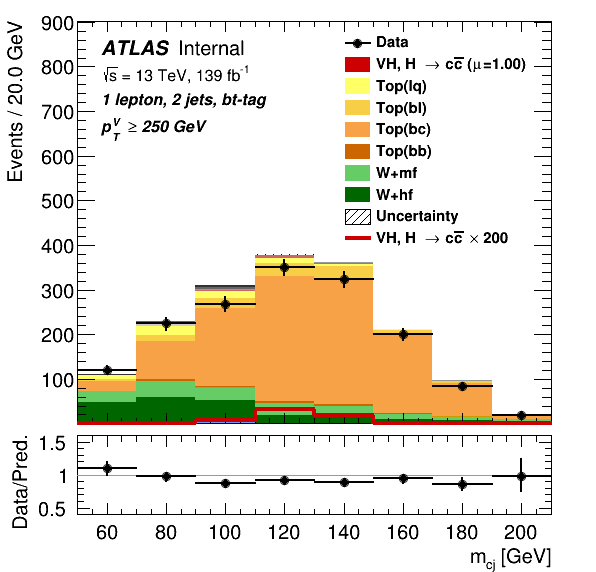
\includegraphics[scale=0.2]{Images/VH/SRsandTopCRs/Region_distmBB_DtopCRBC_L1_Y6051_TTypebt_T1_J2_BMin250_Prefit.png}\\

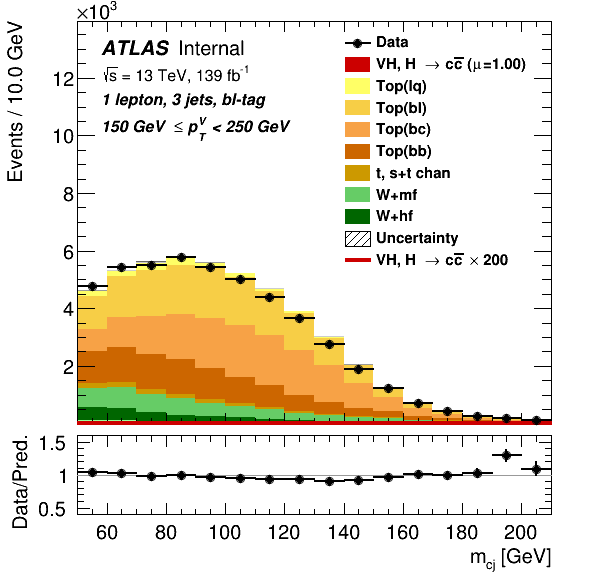
\includegraphics[scale=0.2]{Images/VH/SRsandTopCRs/Region_distmBB_DtopCRBL_BMax250_L1_Y6051_TTypebl_T1_J3_BMin150_Prefit.png}
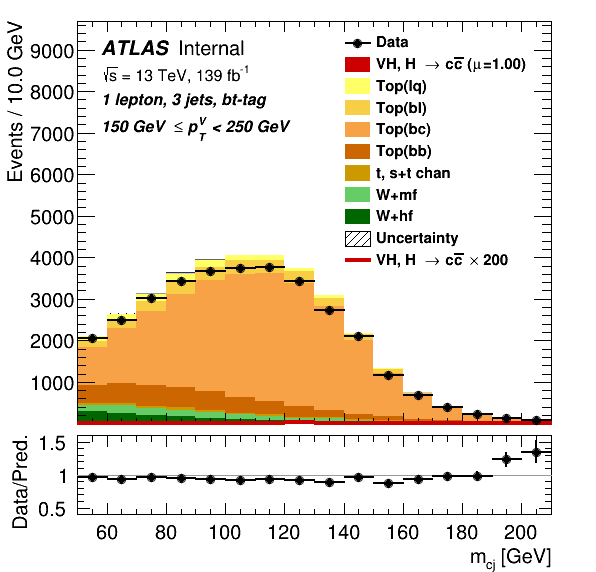
\includegraphics[scale=0.2]{Images/VH/SRsandTopCRs/Region_distmBB_DtopCRBC_BMax250_L1_Y6051_TTypebt_T1_J3_BMin150_Prefit.png}
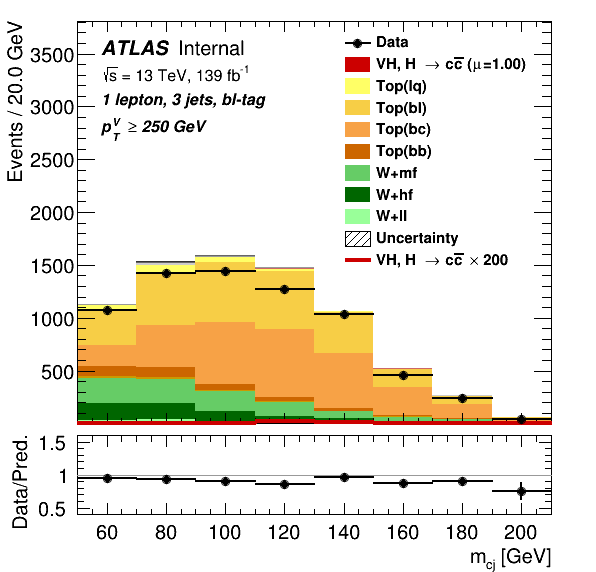
\includegraphics[scale=0.2]{Images/VH/SRsandTopCRs/Region_distmBB_DtopCRBL_L1_Y6051_TTypebl_T1_J3_BMin250_Prefit.png}
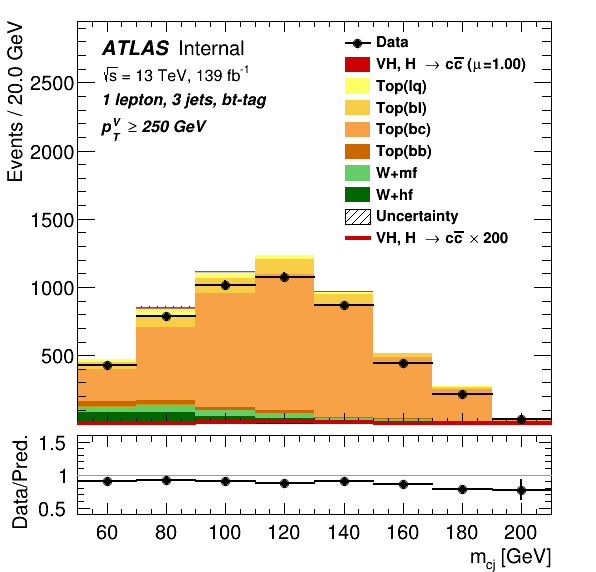
\includegraphics[scale=0.2]{Images/VH/SRsandTopCRs/Region_distmBB_DtopCRBC_L1_Y6051_TTypebt_T1_J3_BMin250_Prefit.png}
\caption{The 1L top control regions $m_{c\bar{c}}$ distributions in both $p_T^V$ ranges (left two columns are [150, 250] GeV, right two are > 250 GeV). Per group of two adjacent: left is BL, right is BT. Top: 2 jets; bottom: 3 jets.} 
\label{fig:topCRslowptv}
\end{figure}

\begin{figure}[h!]
\vspace{0.1cm}
\center
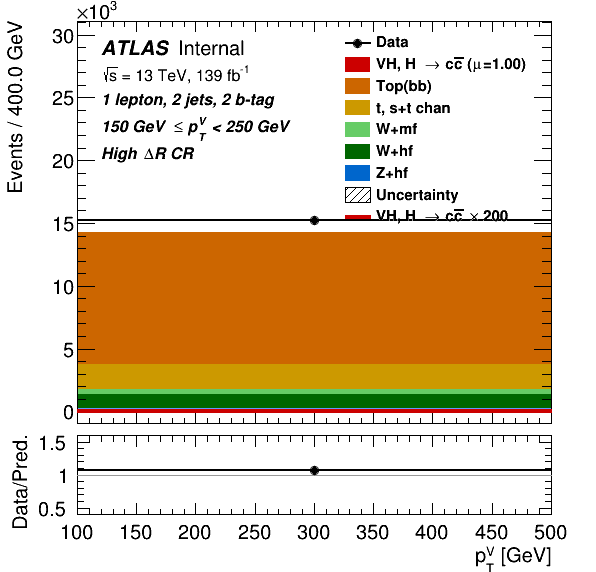
\includegraphics[scale=0.3]{Images/VH/SRsandTopCRs/Region_distpTV_DCRHigh_BMax250_L1_Y6051_TTypebb_T2_J2_BMin150_Prefit.png}
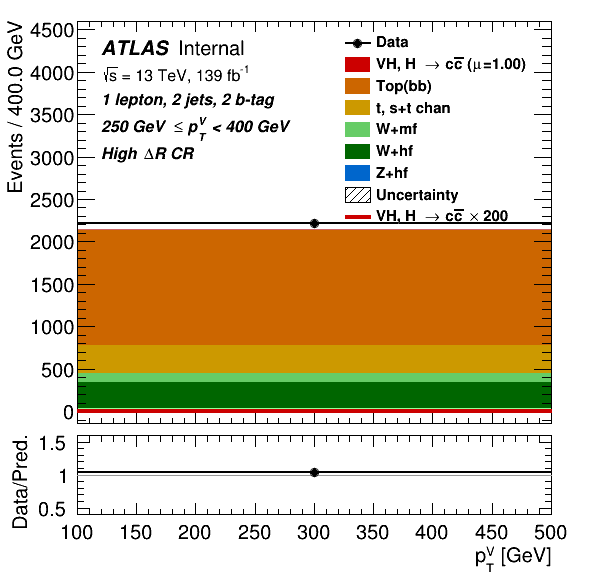
\includegraphics[scale=0.3]{Images/VH/SRsandTopCRs/Region_distpTV_DCRHigh_BMax400_L1_Y6051_TTypebb_T2_J2_BMin250_Prefit.png}\\
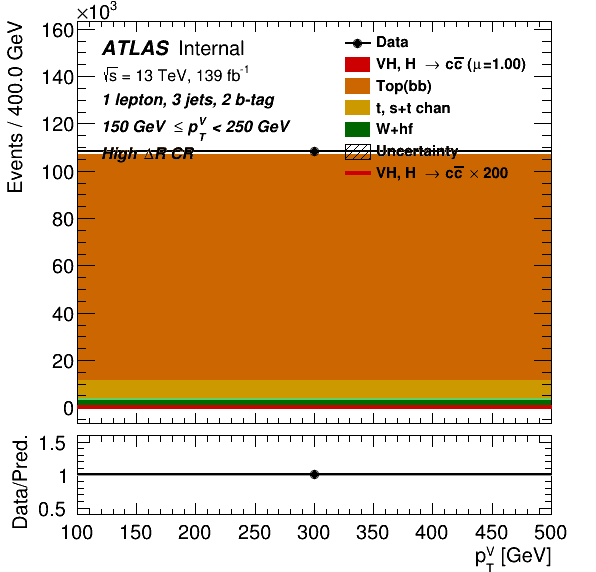
\includegraphics[scale=0.3]{Images/VH/SRsandTopCRs/Region_distpTV_DCRHigh_BMax250_L1_Y6051_TTypebb_T2_J3_BMin150_Prefit.png}
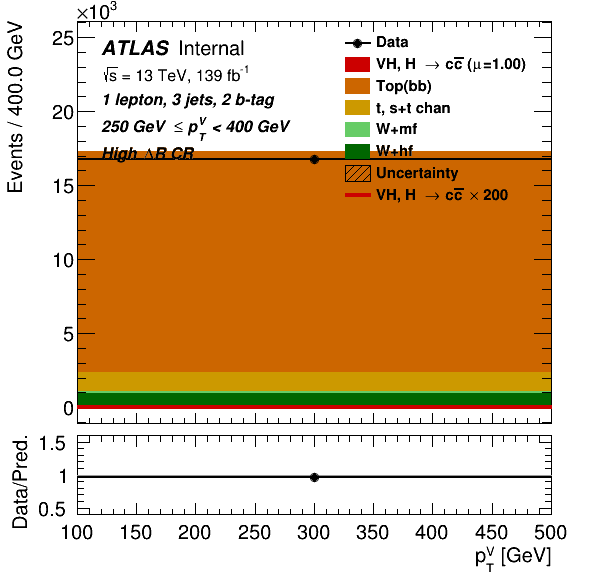
\includegraphics[scale=0.3]{Images/VH/SRsandTopCRs/Region_distpTV_DCRHigh_BMax400_L1_Y6051_TTypebb_T2_J3_BMin250_Prefit.png}
\caption{The 1L 1-bin  $VH(H\rightarrow b\bar{b})$ High $\Delta R$ CR in both $p_T^V$ ranges. Left: [150, 250] GeV; right: [250, 400] GeV. Top: 2 jets; bottom: 3 jets.} 
\label{fig:vhbbDRCR}
\end{figure}

\begin{figure}[h!]
%\hspace{-2.0cm}
\center
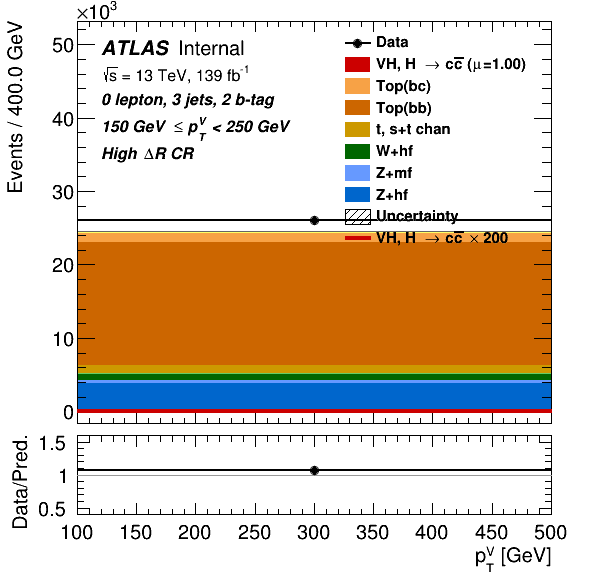
\includegraphics[scale=0.325]{Images/VH/SRsandTopCRs/Region_distpTV_DCRHigh_BMax250_L0_Y6051_TTypebb_T2_J3_BMin150_Prefit.png}
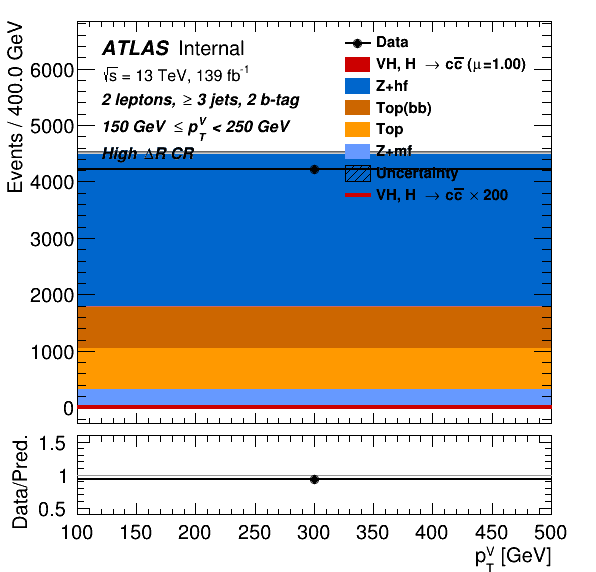
\includegraphics[scale=0.325]{Images/VH/SRsandTopCRs/Region_distpTV_DCRHigh_BMax250_BMin150_Y6051_TTypebb_T2_J3_L2_incJet1_Prefit.png}
\caption{The $VH(H\rightarrow b\bar{b})$ High $\Delta R$ CR in the [150, 250] GeV $p_T^V$ range region with 3 jets, for 0L on the left, and 2L on the right.} 
\label{fig:vhbbDRCR02L}
\end{figure}

For $VH(H\rightarrow c\bar{c})$, the $bc$ and $bl$ components are the most important to constrain. In $VH(H\rightarrow b\bar{b})$, while the $bc$ component is also significant and can benefit from the topCRs, the most important contribution comes from the $bb$ one and is well constrained by the High $\Delta R$ CR, since in a $t\bar{t}$ decay the two produced $b$-jets tend to be separated by a large $\Delta R$ due to the event topology. For the Combined Analysis, the SRs and CRs of both analyses will be considered simultaneously. To show the impact on the $VH(H\rightarrow c\bar{c})$ standalone analysis, the High $\Delta R$ CR from  $VH(H\rightarrow b\bar{b})$ is included to study the effect on the $bc$ and $bl$ components. The aim is to demonstrate these and the $bb$ component can be well constrained with these regions alone, and in particular without the SRs of $VH(H\rightarrow b\bar{b})$. The $VH(H\rightarrow b\bar{b})$ High $\Delta R$ control regions are taken as a single bin of $p_T^V$, because the interest is solely to constrain the top($bb$) normalisation. Figure \ref{fig:vhbbDRCR} displays the 1L $VH(H\rightarrow b\bar{b})$ High $\Delta R$ CR, which is visibly dominated by the top($bb$). Figure \ref{fig:vhbbDRCR02L} shows the same region for the [150, 250] GeV $p_T^V$ range with 3 jets in 0L and 2L, showing a significant proportion of $Z$+jets is also included in these regions.  \\

\subsubsection{Statistical analysis}
After collecting the data and simulating the various samples, including the detector effects, reconstructing the physics objects, and applying the different cuts and the event categorisation, the last step in the analysis is to measure the signal yield normalised to the expected SM yield (from theory, i.e., $\sigma \times BR$). The analysis aims to define a 95\% confidence level on the maximum signal enhancement factor $\mu$. This is done by maximising the binned-likelihood distribution in all of the analysis regions simultaneously as a function of the signal strength and statistical and systematic uncertainties. The full binned-likelihood function can be decomposed into three terms \cite{Mironova:2837159}: 
\begin{enumerate}
\item A Poisson probability term based on the expected and observed event yields in all bins of the considered distributions tracks the signal strength: $\mathcal{L} = \prod_{i\in \textrm{bins}} \textrm{Pois}(N_i \,|\, \mu s_i + b_i)$, where $N_i$, $s_i$, and $b_i$ are respectively the number of measured data events, the expected (simulated) signal yield, and the expected background yield in bin $i$. The signal strength parameter $\mu$ is the ratio of the measured $\sigma \times \textrm{BR}$ divided by the SM expectation for the signal process.  
\item Systematics uncertainties enter the fit as Nuisance Parameters (NP) $\overrightarrow{\theta}$ which can modify the expected signal and background yields $s_i(\overrightarrow{\theta})$ and $b_i(\overrightarrow{\theta})$ in each bin. They are modelled as standardised Gaussian penalty terms: $\mathcal{L_{\textrm{NP}}} = \prod_{\theta \in \overrightarrow{\theta}} \frac{1}{\sqrt{2\pi}} e^{- \theta^2/2}$. After the fit, the values of the NPs can be moved upwards or downwards, and this deviation from 0 (from 1 for the normalisation factors) is called a \textit{pull}. The \textit{constraint} indicates the certainty on the value of the NP after the fit. NPs can have a prior, based on pre-existing knowledge or empirical estimates (e.g. auxiliary measurements, MC simulation model differences), or be left \textit{free-floating} (with a prefit value of 1), such as for the normalisation of the major backgrounds which is determined from data in control regions where these processes are enhanced. 
\item Uncertainties tracking the limited available statistics of the simulations are introduced as $\gamma_i$-parameters, with one such parameter per bin. They give the fit the flexibility to adjust the expected background yield in a particular bin as $b_i(\overrightarrow{\theta}) \rightarrow \gamma_i b_i(\overrightarrow{\theta})$. They are introduced as: $\mathcal{L_{\textrm{BkgStat}}}(\overrightarrow{\gamma}) = \prod_{i \in \textrm{bins}} \textrm{Gauss}(\beta_i | \gamma_i \beta_i, \sqrt{\gamma_i \beta_i})$, where $\beta_i = 1 / \sigma^2_\textrm{rel}$ and $\sigma_\textrm{rel}$ is the relative statistical uncertainty on the expected total background yield. 
\end{enumerate} 
The full likelihood function is then described as the product of these three contributions as 
\begin{equation}
\mathcal{L} = \prod_{i\in \textrm{bins}} \textrm{Pois}(N_i \,|\, \mu s_i(\overrightarrow{\theta}) + \gamma_i b_i(\overrightarrow{\theta})) \times  \prod_{\theta \in \overrightarrow{\theta}} \frac{1}{\sqrt{2\pi}} e^{- \theta^2/2} \times \prod_{i \in \textrm{bins}} \textrm{Gauss}(\beta_i | \gamma_i \beta_i, \sqrt{\gamma_i \beta_i}).
\end{equation}
For the signal, as previously described, a BDT score is used as a discriminant variable. Also called a \textit{Multivariate Analysis Discriminant} (MVA), one such BDT is trained per lepton channel, separately for $VH(H\rightarrow b\bar{b})$ and $VH(H\rightarrow c\bar{c})$. For the topCRs and the $\Delta R$ control regions, the invariant mass of the candidate pair  $m_{c\bar{c}}$ is used. \\

Systematic uncertainties, that act as priors and are constrained in the fit, on the simulated top background events (\textit{nominal samples}) are assessed by comparing the output of different setups of the simulator as well as using alternative simulators. Variations studied in these \textit{alternative samples} concern the matrix element generation (hard scattering), the renormalisation scale $\mu_R$ and factorisation scale $\mu_F$ for the ISR and FSR, the \textit{Parton Shower} (PS), the underlying event simulation, and multiple parton interactions \cite{Mironova:2837159}. Similar uncertainties are introduced for each of the other background processes. In addition, experimental uncertainties that affect all processes are introduced for the triggers, object reconstruction, flavour tagging, and the recorded data luminosity. They cover resolution effects, reconstruction efficiencies, and differences between data and simulations.\\

The different top components normalisations in 0L and 1L are determined from data in the profile likelihood fit by free-floating norm-factors (NF). A prior normalisation uncertainty is applied to account for potential differences between 0L and 1L. Acceptance ratios, in the number of jets and also in the extrapolation from the control region to the signal region, and shape uncertainties are also applied, after being derived for the top background in the 0L and 1L. When two top components are jointly floated, the dominated component is given an extra flavour ratio uncertainty to add flexibility to the fit. For example, when floating top($bl$) with top($bc$), the normalisation is mostly driven by top($bc$), the dominating component, and a ratio $bl$/$bc$ is added to let the $bl$ components adjust to differences between the two.  \\

The objective of this section is to study the impact of the modified top control regions on the combined 012L $VH(H\rightarrow c\bar{c})$ fit. The aim is to study for which top components the fit regions, and in particular the topCRs, provide enough information to determine their normalisation and constrain their shape from data. Furthermore, the data in the SRs should be sufficiently well described using the complete fit setup and the top background control regions should not significantly impact the behaviour (the NPs) of other backgrounds. While every bin of the analysis is used in the fit, bins with a large fraction of the signal (e.g., at high BDT score in the SRs) are not displayed as the analysis is still blinded. \\

Several iterations of the fit studies were performed to test the new topCRs proposed in this work and in particular which components can be constrained and which NPs can be correlated. The correctness of each fit is evaluated by verifying several diagnostics information, such as changes to the constraining of non-top-related NPs and to the predicted postfit yields. In the present report, three setups are presented to represent the evolution of the implementation of the topCR:
\begin{itemize}
\item Nominal: this is the first implementation to use all available topCRs (BT and BL) and the $VH(H\rightarrow b\bar{b})$ High $\Delta R$ CR with minimal changes to the other NPs. Other novelties introduced here are to free-float separately the top($bc$) and top($bl$) and to float the top($bb$) normalisation. The 2-jet and 3-jet regions share the same NFs and an additional 3-to-2-jet extrapolation uncertainty is implemented and applied in 2-jet. TopCR-SR extrapolation uncertainties are applied in the SRs except for top($lq$) where it is applied in the topCR. 
\item Baseline 2: uses only the topCR BT. Compared to the Nominal, the topCR BL is removed as it has a large $V$+jets background, especially in 0L, and impacts the NPs associated with this process, which is not the aim of the top control region. The top($bl$) is now floated jointly with top($bc$), as they are similar physics-wise since they both select a $b$-quark from the top-quark decay and a jet from the subsequent $W$ decay. An extra NP is introduced to model the $bl$ to $bc$ ratio. The main selection difference between the topCRs and the SRs is the tagging criteria. This difference should be covered by the flavour tagging uncertainties and the topCR-SR extrapolation uncertainties are therefore dropped. The flavour components represent different parts of the top components being selected as candidate jets. The difference induced in the 2-jet and 3-jet regions is not expected to be the same between the flavour components, hence the 3-to-2 jet extrapolation is decorrelated by flavour, separately for $t\bar{t}$ and $Wt$, marking the last modification with respect to the nominal setup.
\item Baseline 2 + nJetDec: is similar to Baseline 2 but now the topCR NFs are decorrelated on the number of jets. This is the preferred scenario if the data and CRs are powerful enough for the fit to converge since it maximally exploits the knowledge from the data and altogether avoids the need for 3-to-2 jet extrapolation uncertainties. These latter uncertainties can be very large because they cover different levels of mis-reconstructed or out-of-acceptance objects involved in the distinction of the top background into the 2-jet and 3-jet regions.
\end{itemize}

Figures \ref{fig:pullsTop} and \ref{fig:pullsFTAG} compare the pulls obtained by the different baselines considered. The top of Figure \ref{fig:pullsTop} shows the floating normalisations of the top background. The [150, 250] GeV region is indicated by the \textit{BMin150} suffix and the region above 250 GeV by \textit{BMin250}, while the number of jets region is indicated by a suffix $J2$ or $J3$. All of the top components NFs are well constrained and the values obtained are consistent between the different $p_T^V$ regions and, for Baseline 2+nJetDec (in red), the number of jets regions. One small exception is the top($lq$) in Baseline 2+nJetDec. This component is however less relevant to the analysis and the top($lq$) can simply be kept inclusive in the number of jets in the final setup. Thanks to the inclusion of the CRHigh from $VH(H\rightarrow b\bar{b})$, even the top($bb$) component is well constrained in $VH(H\rightarrow c\bar{c})$. When removing the topCR BL, a small difference is induced in the NF for the V+jets background (not shown in the Figure). For example, the postfit yield of the W+jets background in the 1L [150, 250] GeV TT SR changes by 0.69\% between the Nominal and Baseline 2 + nJetDec (from 461000 to 457800 expected events). \\

\begin{figure}[h!]
%\hspace{-4.0cm}
\vspace{-1.4cm}
\centering
\begin{subfigure}[b]{0.49\textwidth}
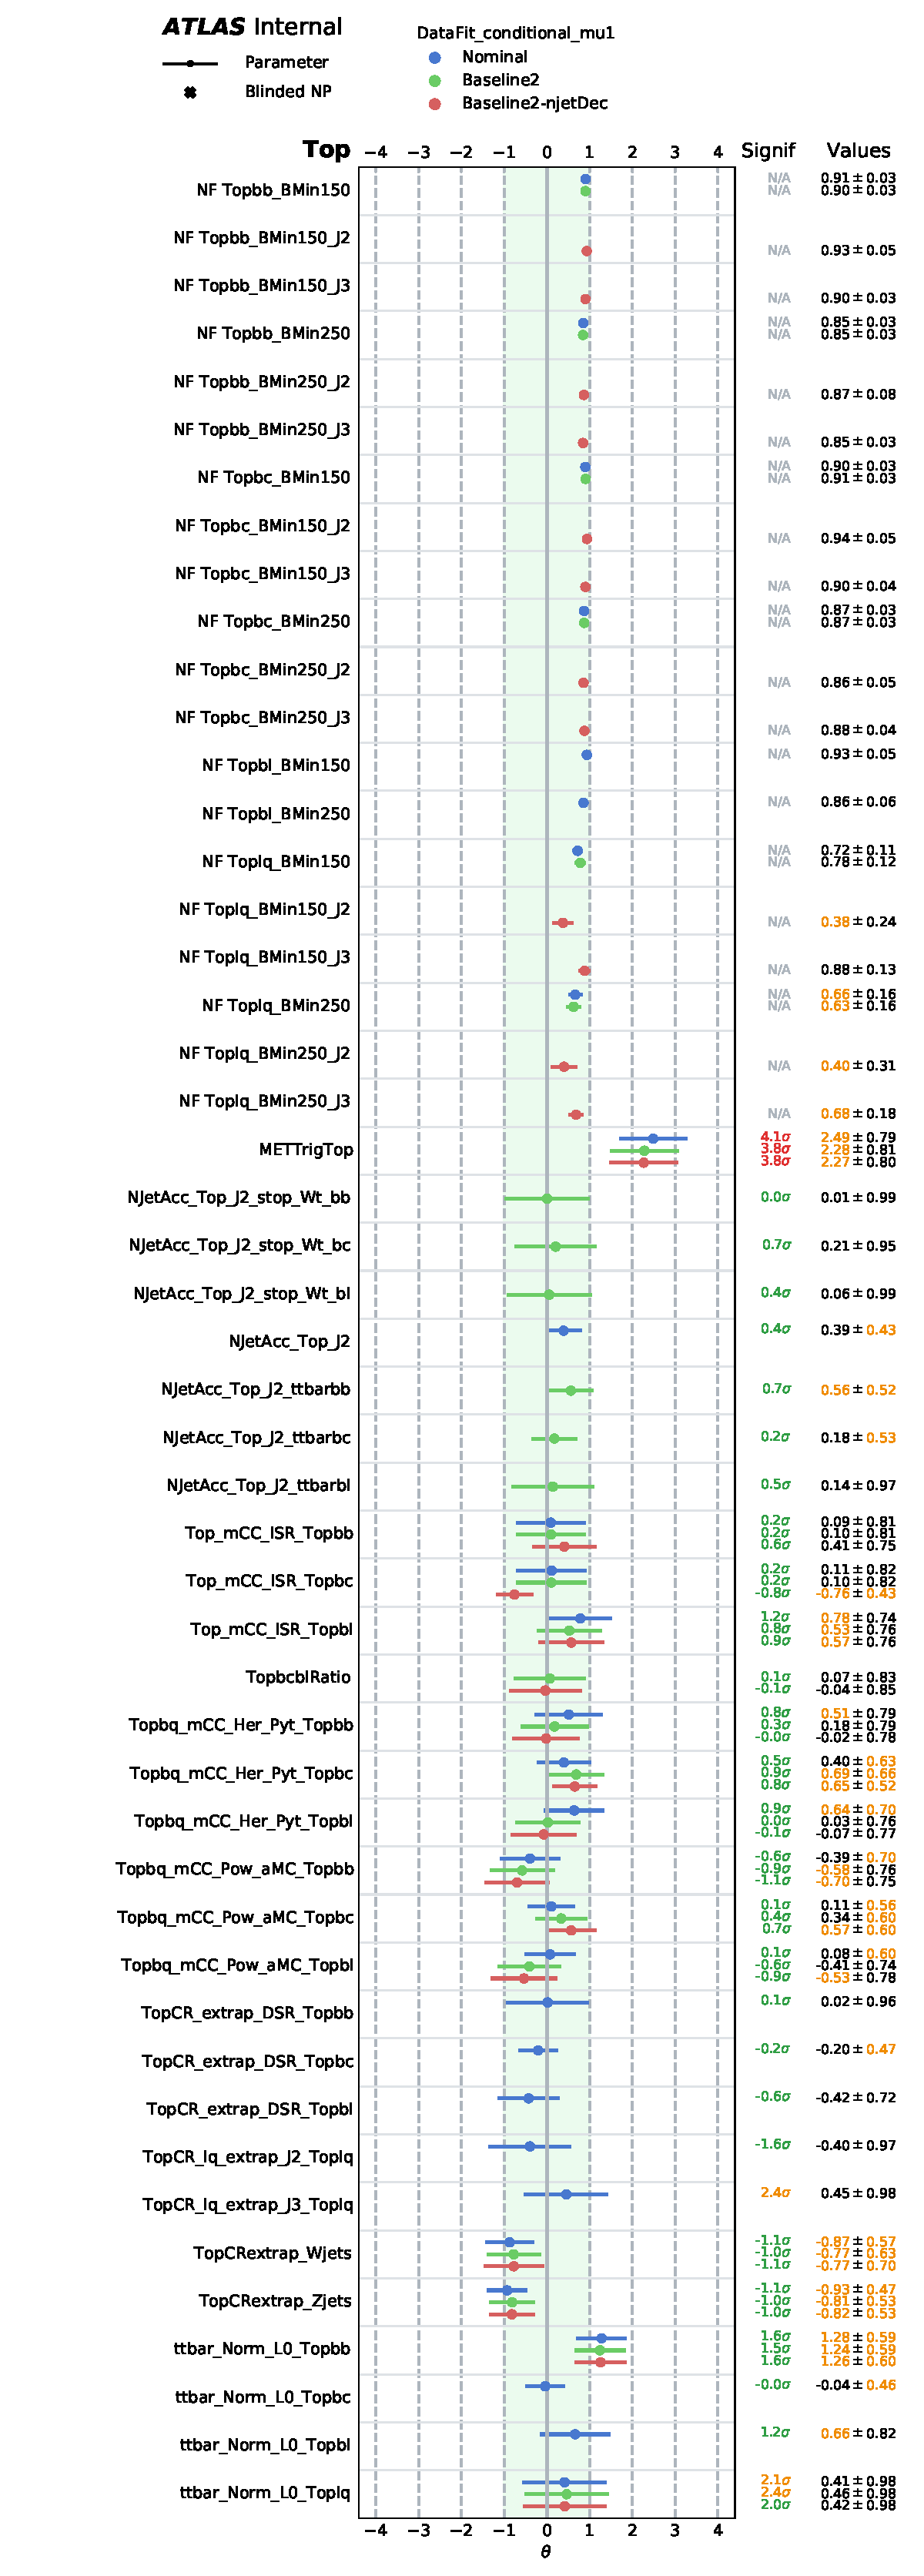
\includegraphics[scale=0.43]{Images/VH/clean_pull/NP_Top.pdf}
\caption{Top pulls.} 
\label{fig:pullsTop}
\end{subfigure}
 %
 \hfill
 %
\begin{subfigure}[b]{0.49\textwidth}
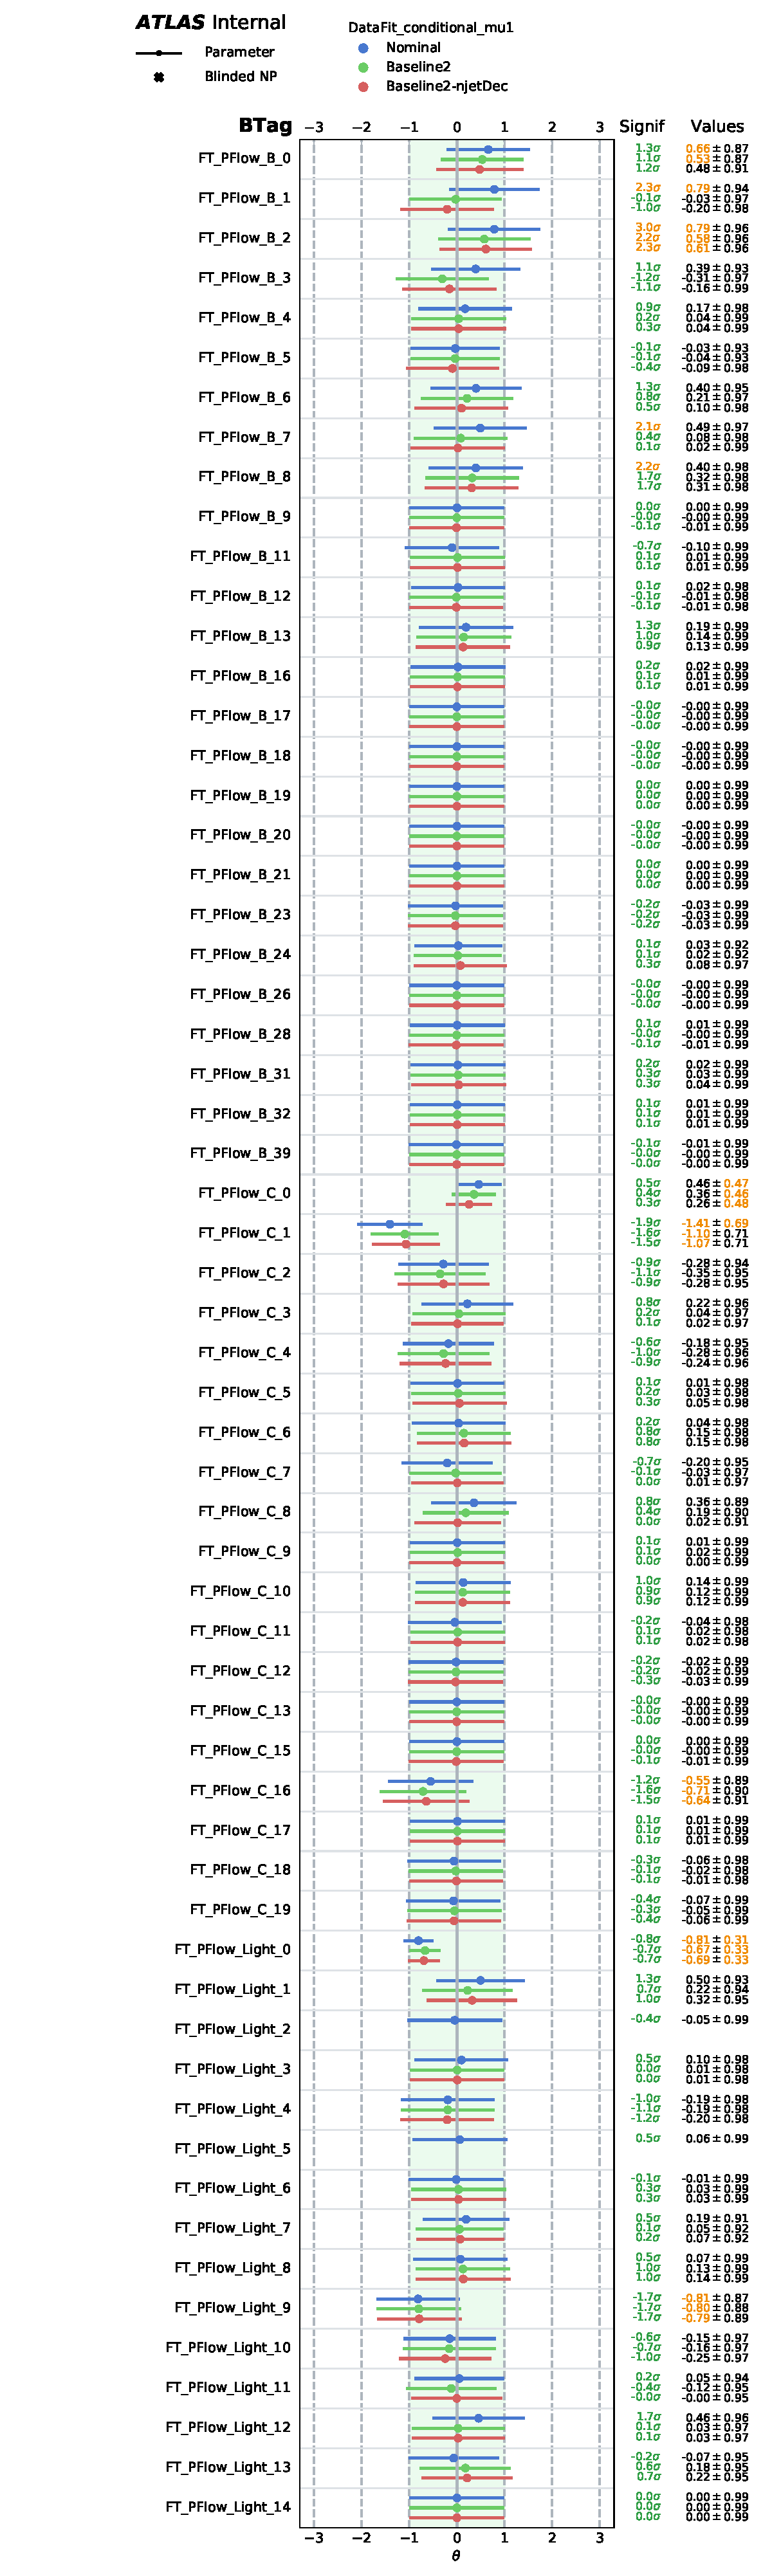
\includegraphics[scale=0.36]{Images/VH/clean_pull/NP_BTag.pdf}
\caption{Flavour tagging pulls.} 
\label{fig:pullsFTAG}
\end{subfigure}
\caption{Pulls for the 012L fit with the several baselines. Blue: nominal; green: baseline 2; red: baseline 2 + nJetDec.}
\label{fig:pulls}
\end{figure} 

The rest of Figure \ref{fig:pullsTop} shows the most important top-related NPs. The METTrigTop, covering the differences between data and simulation in the MET trigger efficiency for top processes, is strongly pulled for all fit setups, something that requires further investigation from the analysis team. The NPs with name of the form \textit{NJetAcc\_Top*} list the nJet acceptances, a single one for the Nominal in blue and split in flavour for Baseline 2 in green. They are removed in Baseline 2 + nJetDec as in this case the NFs are floated separately for each number of jets region. This last setup is able to avoid incurring the rather large systematics induced by these 3-to-2 jets extrapolation uncertainties. Underneath the nJet acceptances, the pulls with names starting with \textit{Top\_mCC} represent shape systematics derived by considering the difference between the nominal samples and the alternative generators (such as Herwig and Powheg) or internal variations (like for the ISR). The $topCR\_extrap$ are the topCR-SR extrapolation uncertainties which are only applied in the Nominal setup. For the Baseline 2 variations, the flavour tagging NPs and associated pulls are able to cover this extrapolation with minimal changes to the Nominal, as shown in Figure \ref{fig:pullsFTAG}. Through these different groups, the interesting observation is that the Baseline 2 + nJetDec performs similarly to the Baseline 2 and Nominal, despite having a much simpler structure without nJet acceptances nor topCR extrapolations. A closer look at other NPs, such as the b-tagging pulls, confirms there is a good agreement between the different alternatives and no over-constraining is observed. \\

The expected prefit 95\% confidence limits on the signal strength of $VH(H\rightarrow c\bar{c})$ of these conditional data fits are: 
\begin{itemize}
\item Nominal: $12.60^{+4.94}_{-3.52}$ × SM
\item Baseline 2: $12.75^{+4.99}_{-3.56}$ × SM
\item Baseline 2 + nJetDec: $12.71^{+4.98}_{-3.55}$ × SM
\end{itemize}
These values are consistent between the different fits. Comparing the fit setups, Baseline 2 + nJetDec is preferred to serve as a new nominal thanks to its simplified fit structure, its lower number of NPs and normalisation factors, the ability to constrain the components in several number of jet regions, and the freedom to use the topCR BL region as a validation region rather than as a control region. The obtained limits are significantly improved compared to the previous ATLAS result of 26 × SM (31 × SM) \cite{Collaboration:2721696} and are competitive with the recent CMS results of an observed (expected) upper limit of 14 $\times$ SM (7.6 $\times$ SM) \cite{arXiv:2205.05550}. The analysis is however still not concluded and improvements are still being pursued by fine-tuning the event selection to avoid large uncertainties as much as possible, including new MC samples with lower MC statistical uncertainties, as well as revisiting the modelling uncertainties all while monitoring the fit behaviour and carrying out similar studies to the present one for other regions and backgrounds. 

\subsection{Conclusion}
The $VH(H\rightarrow b\bar{b}/c\bar{c})$ analysis of Run 2 provides an exciting avenue to improve the competitivity of the ATLAS measurement of the charm Yukawa coupling. While the analysis is still ongoing, the harmonisation of the $VH(H\rightarrow b\bar{b})$ and $VH(H\rightarrow c\bar{c})$, the refinement of the top control region, the introduction of MVA sas discriminating variables, and the many other modifications pursued in the Combined Analysis already indicate significant gains will be made on the previously published result. The analysis is planned to wrap up in the following months and will be described in detail in the final DPhil dissertation. 

\clearpage

